\documentclass[11pt,reqno]{amsart}

\usepackage{amsfonts, amsthm, amsmath, amssymb}
\allowdisplaybreaks[4]

\usepackage{tikz} %\UTF{7ED8}\UTF{56FE}%

\usepackage{float} %使用浮\UTF{52A8}体(表格、\UTF{56FE}片)
\usepackage{multirow} %表格\UTF{7EB5}向合并\UTF{5355}元格
\usepackage{supertabular} %制作超\UTF{8FC7}一\UTF{9875}的表格

%定\UTF{4E49}\UTF{7F57}\UTF{9A6C}数字
\makeatletter
\newcommand{\rmnum}[1]{\romannumeral #1}
\newcommand{\Rmnum}[1]{\expandafter\@slowromancap\romannumeral #1@}
\makeatother

\usepackage{enumerate} %列表\UTF{73AF}境
\usepackage[inline]{enumitem} %列表\UTF{7F16}号

\usepackage[pagebackref]{hyperref} %超\UTF{94FE}接功能, pagebackref\UTF{5B9E}\UTF{73B0}参考文献与正文的双向\UTF{94FE}接
\hypersetup{colorlinks=true} %取消超\UTF{94FE}接\UTF{8FB9}框,\UTF{94FE}接文字\UTF{5E26}\UTF{989C}色

\usepackage{mathabx}

\numberwithin{equation}{section}
\topmargin 0.8in
\textheight=8.2in
\textwidth=6.4in
\voffset=-.68in
\hoffset=-.68in
%\renewcommand{\baselinestretch}{1.2}
\def\numset#1{{\mathbb #1}}
\def\blue{\textcolor{blue}}
\def\red{\textcolor{red}}
\def\magenta{\textcolor{magenta}}
\theoremstyle{plain}

\newtheorem{theorem}{Theorem}[section]
\newtheorem{lemma}[theorem]{Lemma}
\newtheorem{corollary}[theorem]{Corollary}
\newtheorem{St}[theorem]{Statement}
\newtheorem{claim}[theorem]{Claim}
\newtheorem{proposition}[theorem]{Proposition}
\newtheorem{Fact}[theorem]{Fact}
\theoremstyle{definition}
\newtheorem{Def}[theorem]{Definition}
\newtheorem{example}[theorem]{Example}
\newtheorem{conj}[theorem]{Conjecture}
\newtheorem{remark}[theorem]{Remark}
\newtheorem{?}[theorem]{Problem}

\newcommand{\SF}[1]{\color{magenta}#1}

%%% Notations
\newcommand{\A}{\mathcal{A}}
\newcommand{\B}{\mathcal{B}}
\newcommand{\D}{\mathcal{D}}
\renewcommand{\L}{\mathcal{L}}
\renewcommand{\P}{\mathcal{P}}
\renewcommand{\S}{\mathfrak{S}}
\newcommand{\W}{\mathcal{W}}
\def\des{\mathrm{des}}
\def\std{\mathrm{std}}
\def\st{\mathrm{st}}
\def\inv{\mathrm{inv}}
\def\blk{\mathrm{blk}}
\def\sing{\mathrm{sing}}
\def\Par{\mathrm{Par}}

\begin{document}

\title[Consecutive and quasi-consecutive patterns]{Consecutive and quasi-consecutive patterns: $\mathrm{des}$-Wilf classifications and generating functions}


\author[Y. Wang, Q.Fang, S. Fu, S. Kitaev, H. Li]{Yan Wang, Qi Fang, Shishuo Fu, Sergey Kitaev, Haijun Li}
\address[Yan Wang]{College of Mathematics and Statistics, Chongqing University, Chongqing 401331, P.R. China}
\email{yanw2143@foxmail.com}
\address[Qi Fang]{College of Mathematics and Statistics, Chongqing University, Chongqing 401331, P.R. China}
\email{qifangpapers@163.com}
\address[Shishuo Fu]{College of Mathematics and Statistics, Chongqing University, Chongqing 401331, P.R. China}
\email{fsshuo@cqu.edu.cn}
\address[Sergey Kitaev]{Department of Mathematics and Statistics, University of Strathclyde, 26 Richmond Street, Glasgow G1 1XH, UK}
\email{sergey.kitaev@strath.ac.uk}
\address[Haijun Li]{College of Mathematics and Statistics, Chongqing University, Chongqing 401331, P.R. China}
\email{lihaijun@cqu.edu.cn}

\date{\today}

\begin{abstract}
Motivated by a correlation between the distribution of descents over permutations that avoid a consecutive pattern and those avoiding the respective quasi-consecutive pattern, as established in this paper, we obtain a complete $\des$-Wilf classification for quasi-consecutive patterns of length up to 4. For equivalence classes containing more than one pattern, we construct various descent-preserving bijections to establish the equivalences, which lead to the provision of proper versions of two incomplete bijective arguments previously published in the literature. Additionally, for two singleton classes, we derive explicit bivariate generating functions using the generalized run theorem.
\end{abstract}

\maketitle

\section{Introduction}

\section{Introduction}
\label{sec:introduction}
The business processes of organizations are experiencing ever-increasing complexity due to the large amount of data, high number of users, and high-tech devices involved \cite{martin2021pmopportunitieschallenges, beerepoot2023biggestbpmproblems}. This complexity may cause business processes to deviate from normal control flow due to unforeseen and disruptive anomalies \cite{adams2023proceddsriftdetection}. These control-flow anomalies manifest as unknown, skipped, and wrongly-ordered activities in the traces of event logs monitored from the execution of business processes \cite{ko2023adsystematicreview}. For the sake of clarity, let us consider an illustrative example of such anomalies. Figure \ref{FP_ANOMALIES} shows a so-called event log footprint, which captures the control flow relations of four activities of a hypothetical event log. In particular, this footprint captures the control-flow relations between activities \texttt{a}, \texttt{b}, \texttt{c} and \texttt{d}. These are the causal ($\rightarrow$) relation, concurrent ($\parallel$) relation, and other ($\#$) relations such as exclusivity or non-local dependency \cite{aalst2022pmhandbook}. In addition, on the right are six traces, of which five exhibit skipped, wrongly-ordered and unknown control-flow anomalies. For example, $\langle$\texttt{a b d}$\rangle$ has a skipped activity, which is \texttt{c}. Because of this skipped activity, the control-flow relation \texttt{b}$\,\#\,$\texttt{d} is violated, since \texttt{d} directly follows \texttt{b} in the anomalous trace.
\begin{figure}[!t]
\centering
\includegraphics[width=0.9\columnwidth]{images/FP_ANOMALIES.png}
\caption{An example event log footprint with six traces, of which five exhibit control-flow anomalies.}
\label{FP_ANOMALIES}
\end{figure}

\subsection{Control-flow anomaly detection}
Control-flow anomaly detection techniques aim to characterize the normal control flow from event logs and verify whether these deviations occur in new event logs \cite{ko2023adsystematicreview}. To develop control-flow anomaly detection techniques, \revision{process mining} has seen widespread adoption owing to process discovery and \revision{conformance checking}. On the one hand, process discovery is a set of algorithms that encode control-flow relations as a set of model elements and constraints according to a given modeling formalism \cite{aalst2022pmhandbook}; hereafter, we refer to the Petri net, a widespread modeling formalism. On the other hand, \revision{conformance checking} is an explainable set of algorithms that allows linking any deviations with the reference Petri net and providing the fitness measure, namely a measure of how much the Petri net fits the new event log \cite{aalst2022pmhandbook}. Many control-flow anomaly detection techniques based on \revision{conformance checking} (hereafter, \revision{conformance checking}-based techniques) use the fitness measure to determine whether an event log is anomalous \cite{bezerra2009pmad, bezerra2013adlogspais, myers2018icsadpm, pecchia2020applicationfailuresanalysispm}. 

The scientific literature also includes many \revision{conformance checking}-independent techniques for control-flow anomaly detection that combine specific types of trace encodings with machine/deep learning \cite{ko2023adsystematicreview, tavares2023pmtraceencoding}. Whereas these techniques are very effective, their explainability is challenging due to both the type of trace encoding employed and the machine/deep learning model used \cite{rawal2022trustworthyaiadvances,li2023explainablead}. Hence, in the following, we focus on the shortcomings of \revision{conformance checking}-based techniques to investigate whether it is possible to support the development of competitive control-flow anomaly detection techniques while maintaining the explainable nature of \revision{conformance checking}.
\begin{figure}[!t]
\centering
\includegraphics[width=\columnwidth]{images/HIGH_LEVEL_VIEW.png}
\caption{A high-level view of the proposed framework for combining \revision{process mining}-based feature extraction with dimensionality reduction for control-flow anomaly detection.}
\label{HIGH_LEVEL_VIEW}
\end{figure}

\subsection{Shortcomings of \revision{conformance checking}-based techniques}
Unfortunately, the detection effectiveness of \revision{conformance checking}-based techniques is affected by noisy data and low-quality Petri nets, which may be due to human errors in the modeling process or representational bias of process discovery algorithms \cite{bezerra2013adlogspais, pecchia2020applicationfailuresanalysispm, aalst2016pm}. Specifically, on the one hand, noisy data may introduce infrequent and deceptive control-flow relations that may result in inconsistent fitness measures, whereas, on the other hand, checking event logs against a low-quality Petri net could lead to an unreliable distribution of fitness measures. Nonetheless, such Petri nets can still be used as references to obtain insightful information for \revision{process mining}-based feature extraction, supporting the development of competitive and explainable \revision{conformance checking}-based techniques for control-flow anomaly detection despite the problems above. For example, a few works outline that token-based \revision{conformance checking} can be used for \revision{process mining}-based feature extraction to build tabular data and develop effective \revision{conformance checking}-based techniques for control-flow anomaly detection \cite{singh2022lapmsh, debenedictis2023dtadiiot}. However, to the best of our knowledge, the scientific literature lacks a structured proposal for \revision{process mining}-based feature extraction using the state-of-the-art \revision{conformance checking} variant, namely alignment-based \revision{conformance checking}.

\subsection{Contributions}
We propose a novel \revision{process mining}-based feature extraction approach with alignment-based \revision{conformance checking}. This variant aligns the deviating control flow with a reference Petri net; the resulting alignment can be inspected to extract additional statistics such as the number of times a given activity caused mismatches \cite{aalst2022pmhandbook}. We integrate this approach into a flexible and explainable framework for developing techniques for control-flow anomaly detection. The framework combines \revision{process mining}-based feature extraction and dimensionality reduction to handle high-dimensional feature sets, achieve detection effectiveness, and support explainability. Notably, in addition to our proposed \revision{process mining}-based feature extraction approach, the framework allows employing other approaches, enabling a fair comparison of multiple \revision{conformance checking}-based and \revision{conformance checking}-independent techniques for control-flow anomaly detection. Figure \ref{HIGH_LEVEL_VIEW} shows a high-level view of the framework. Business processes are monitored, and event logs obtained from the database of information systems. Subsequently, \revision{process mining}-based feature extraction is applied to these event logs and tabular data input to dimensionality reduction to identify control-flow anomalies. We apply several \revision{conformance checking}-based and \revision{conformance checking}-independent framework techniques to publicly available datasets, simulated data of a case study from railways, and real-world data of a case study from healthcare. We show that the framework techniques implementing our approach outperform the baseline \revision{conformance checking}-based techniques while maintaining the explainable nature of \revision{conformance checking}.

In summary, the contributions of this paper are as follows.
\begin{itemize}
    \item{
        A novel \revision{process mining}-based feature extraction approach to support the development of competitive and explainable \revision{conformance checking}-based techniques for control-flow anomaly detection.
    }
    \item{
        A flexible and explainable framework for developing techniques for control-flow anomaly detection using \revision{process mining}-based feature extraction and dimensionality reduction.
    }
    \item{
        Application to synthetic and real-world datasets of several \revision{conformance checking}-based and \revision{conformance checking}-independent framework techniques, evaluating their detection effectiveness and explainability.
    }
\end{itemize}

The rest of the paper is organized as follows.
\begin{itemize}
    \item Section \ref{sec:related_work} reviews the existing techniques for control-flow anomaly detection, categorizing them into \revision{conformance checking}-based and \revision{conformance checking}-independent techniques.
    \item Section \ref{sec:abccfe} provides the preliminaries of \revision{process mining} to establish the notation used throughout the paper, and delves into the details of the proposed \revision{process mining}-based feature extraction approach with alignment-based \revision{conformance checking}.
    \item Section \ref{sec:framework} describes the framework for developing \revision{conformance checking}-based and \revision{conformance checking}-independent techniques for control-flow anomaly detection that combine \revision{process mining}-based feature extraction and dimensionality reduction.
    \item Section \ref{sec:evaluation} presents the experiments conducted with multiple framework and baseline techniques using data from publicly available datasets and case studies.
    \item Section \ref{sec:conclusions} draws the conclusions and presents future work.
\end{itemize}


\section{Structure Theorem and classification of length-3 quasi-consecutive patterns}\label{sec:structure theorem}

\subsection{Proof of Theorem~\ref{structure thm}}
We begin with a proof of Theorem~\ref{structure thm}, and then collect a few preliminary results for later use.

\begin{proof}[Proof of Theorem~\ref{structure thm}]
    Given a permutation $\pi\in \S_{n+1}(p)$, suppose it has the decomposition $\pi=\pi'(n+1)\pi''$ as shown in Fig.~\ref{fig:decomposition of pi(p)}, where the black dot represents the element $n+1$ in $\pi$, while the left square labeled $A^{\sigma}$ refers to the permutation $\pi'$ of
    length $i\,(0\le i\le n)$, and the right square labeled $A^p$ refers to the permutation $\pi''$. The key observation is that $\pi$ is $p$-avoiding if and only if $\pi'$ is $\sigma$-avoiding and $\pi''$ is $p$-avoiding. Consequently, by considering all possible $i$, we have, for $n\ge 0$,
    \begin{equation}\label{eqn-1}
    A_{n+1}^p(t)=t\sum_{i=0}^{n-1}\binom{n}{i}A_i^{\sigma}(t)A_{n-i}^p(t)+A_n^{\sigma}(t).\end{equation}

    \begin{figure}[ht]
        \centering
        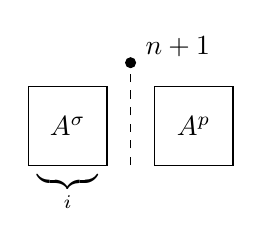
\begin{tikzpicture}
            \draw (-6,5) rectangle (-5,4);
            \fill (-4.7,5.3) circle[radius=2pt];
            \node at (-4.1,5.5) {$n+1$};
            \draw (-4.4,5) rectangle (-3.4,4);
            \draw[dashed] (-4.7,4) -- (-4.7,5.3);
            \node at (-5.5,4.5) {$A^{\sigma}$};
            \node at (-3.9,4.5) {$A^p$};
            \node at (-5.5,3.8) {$\underbrace{\phantom{a+b}}_i$ };
        \end{tikzpicture}
        \caption{A decomposition of $\pi \in \S_{n+1}(p)$}
        \label{fig:decomposition of pi(p)}
    \end{figure}

\noindent
Then, multiplying by $\dfrac{x^n}{n!}$ both sides of (\ref{eqn-1}) and summing over all $n\geq 0$, we obtain
    \begin{align*}
        \sum_{n\ge 0}\frac{A_{n+1}^p(t)x^n}{n!} &= t\sum_{n\ge 0}\sum_{i=0}^{n-1}\frac{A_i^{\sigma}(t)x^i}{i!}\frac{A_{n-i}^p(t)x^{n-i}}{(n-i)!}+\sum_{n\ge 0}A_n^{\sigma}(t)\frac{x^n}{n!} \\
        &= t\sum_{n\ge 0}\sum_{i=0}^{n}\frac{A_i^{\sigma}(t)x^i}{i!}\frac{A_{n-i}^p(t)x^{n-i}}{(n-i)!}-t\sum_{n\ge0}A_n^{\sigma}(t)\frac{x^n}{n!}+\sum_{n\ge 0}A_n^{\sigma}(t)\frac{x^n}{n!} \\
        &= tA^{\sigma}(x,t)A^p(x,t) -tA^{\sigma}(x,t)+A^{\sigma}(x,t).
    \end{align*}

    It follows that $$\sum_{n\ge 0}\frac{A_{n+1}^p(t)x^n}{n!}=\frac{{\partial A^p}}{\partial x}=tA^{\sigma}A^p+(1-t)A^{\sigma}=tA^{\sigma}\left(A^p-1+\frac{1}{t}\right),$$
    where we abbreviate $A^{\sigma}(x,t)$ (resp., $A^p(x,t)$) as $A^{\sigma}$ (resp., $A^p$).
    Setting $\widetilde{A^p}=A^{p}-1+\dfrac{1}{t}$, the initial condition becomes $\widetilde{A^p}(0,t)=\dfrac{1}{t}$ since $A^p(0,t)=1$, and 
    we get $\dfrac{\partial \widetilde{A^p}}{\partial x}=tA^{\sigma}\widetilde{A^p}.$
    Solving this equation with the initial condition, we have 
    $\ln \widetilde{A^p}-\ln \dfrac{1}{t}=t \int_{0}^{x} A^{\sigma}(y,t) \,dy$, and 
    $\widetilde{A^p} = \dfrac{1}{t} e^{t \int_{0}^{x} A^{\sigma}(y,t) \,dy}$.
    Therefore, $A^p = \dfrac{1}{t} e^{t \int_{0}^{x} A^{\sigma}(y,t) \,dy} +1-\dfrac{1}{t}=\dfrac{1}{t} (e^{t \int_{0}^{x} A^{\sigma}(y,t) \,dy}-1) +1$.
\end{proof}

The following result immediately follows from the Structure Theorem, and is useful when we consider the $\des$-Wilf-equivalences for various patterns. It also strengthens Theorem~\ref{thm:eli-kit}.

\begin{corollary}\label{col:structure}
    $\sigma\overset{\des}{\sim}\sigma'$ if and only if $\sigma k\overset{\des}{\sim}\sigma' k$, where $\sigma$ and $\sigma'$ are two consecutive patterns on $\{1,2,\ldots,k-1\}$.
\end{corollary}

Note that the three trivial bijections give rise to obvious Wilf-equivalences such as $123\sim 321$. When we consider $\des$-Wilf-equivalences however, the following result will be handy. For any vincular pattern $\omega$, we abuse the notation and still use $\omega^c$ to denote the vincular pattern whose underlying permutation is the complement of the underlying permutation of $\omega$ with the same set of positions being underlined. For instance, $(\underline{231}4 )^c=\underline{324}1$ and $(\underline{21}4\underline{53})^c=\underline{45}2\underline{13}$. The reverse $\omega^r$ and the reverse-complement $\omega^{cr}=\omega^{rc}$ are understood similarly. So, for example,  $(\underline{231}4 )^r=4\underline{132}$ and $(\underline{21}4\underline{53})^{rc}=\underline{31}2\underline{54}$.

\begin{proposition} \label{omega--omega^rc}
    Let $\omega$ be a vincular pattern, then $\omega \overset{\des}{\sim} \omega^{rc}$, or equivalently $\omega^c \overset{\des}{\sim} \omega^{r}$.
\end{proposition}

\begin{proof}
    It is easily seen that $\des(\pi^{rc})=n-1-\des(\pi^r)=n-1-(n-1-\des(\pi))=\des(\pi)$.
    This indicates that the composition map $\phi_c\circ\phi_r$ preserves the permutation statistic $\des$. Moreover, $\pi \in \S_n(\omega )$ if and only if $\pi^{rc} \in \S_n(\omega^{rc} )$.
    Hence $\omega \overset{\des}{\sim} \omega^{rc}$.
\end{proof}

The following fact will facilitate our derivations of generating functions.

\begin{proposition} \label{omega--omega^c}
    Let $\omega$ be a vincular pattern, then $A^{\omega^c}(x,t)=A^{\omega^r}(x,t)=\dfrac{1}{t} (A^{\omega}(xt,\dfrac{1}{t})-1)+1$.
\end{proposition}

\begin{proof}
    Note that $\des(\pi ^c)=n-1-\des(\pi)$ for $n\ge 1$, and $\pi \in \S_n(\omega) $ if and only if $\pi ^c \in \S_n(\omega^c)$.
    It follows that
    \begin{align*}
        A^{\omega^c}(x,t)&=\sum_{n\ge 0} \sum_{\pi\in \S_n(\omega ^c)} t ^{\des (\pi)}\dfrac{x^n}{n!} \\
        &= \sum_{n\ge 0} \sum_{\pi^c \in \S_n(\omega ^c)} t ^{\des (\pi^c)}\dfrac{x^n}{n!}\\
        &=1+ \sum_{n\ge 1} \sum_{\pi \in \S_n(\omega )} t ^{n-1-\des (\pi)}\dfrac{x^n}{n!}  \\
        &=1+\dfrac{1}{t} \left(A^{\omega}(xt,\dfrac{1}{t})-1\right).
    \end{align*}
   By Proposition~\ref{omega--omega^rc}, $\omega^r \overset{\des}{\sim} \omega^{c}$. Hence, $A^{\omega^c}(x,t) = A^{\omega^r}(x,t)$, completing the proof.
\end{proof}

% Though $\omega$ and $\omega^c$ are not $\des$-Wilf-equivalent, we only need to compute
% the generating function $A^{\omega}(x,t)$ then we naturally know $A^{\omega^c}(x,t)$.


\subsection{Classifications for lengths 2 and 3}

We now provide the complete $\des$-Wilf classification for quasi-consecutive patterns $p = \sigma j$ of length 2 or 3. Using the Structure Theorem, we compute the generating functions $A^p(x, t)$ for all possible choices of $p$, except for $p = \underline{13}2$ and $p = \underline{31}2$. The case of length 2 patterns, $p = \underline{1}2$ and $p = \underline{2}1$, is trivial, as each class contains a unique permutation: $12\cdots n \in \S_n(\underline{2}1)$ and $n(n-1)\cdots 1 \in \S_n(\underline{1}2)$. Their generating functions are straightforward to derive and are included in Table~\ref{tab:2 and 3} for completeness.

% By Proposition~\ref{omega--omega^c}, we only compute the generating function for $\frac{2!}{2}+\frac{3!}{2}=4$ patterns.
% The generating functions about pattern $\sigma k$ of lenth $2$ or $3$ with $\des$ are summarized below.


\begin{table}[h!]
    \setlength{\tabcolsep}{15pt}    %\UTF{8C03}整列\UTF{5BBD}%
    \renewcommand{\arraystretch}{1.2}   %\UTF{8C03}整行距
    \begin{center}
     \begin{tabular}{c|c|c} % <-- Alignments: 1st column left, 2nd middle and 3rd right, with  vertical lines in between
        Pattern $\sigma j$  & $A^{\sigma j}(x,t)$ or $B^{\sigma j}(x,t)$ & Proved in \\ \hline 
        $\underline{1}2$ & $\dfrac{1}{t}(e^{tx}-1)+1$ & N/A  \\ %\hline
        $\underline{2}1$ & $e^{x}$ & N/A  \\ %\hline
        $\underline{12}3$ & $\dfrac{1}{t} (e^{\frac{1}{t}(e^{tx}-1)+x(t-1)}-1)+1$ & Theorem~\ref{thm:12-3 and 21-3} \\ %\hline
        $\underline{32}1$ & $e^{t(e^{x}-1)+x(1-t)}$ & Corollary~\ref{cor:32-1 and 23-1} \\ %\hline
        $\underline{21}3$ & $\dfrac{1}{t} (e^{t(e^x-1)}-1)+1$ & Theorem~\ref{thm:12-3 and 21-3} \\ %\hline
        $\underline{23}1$ & $e^{\frac{1}{t}(e^{xt}-1)}$ &  Corollary~\ref{cor:32-1 and 23-1} \\ %\hline
        $\underline{13}2$, $\underline{31}2$ & $\dfrac{1+x(t-1)-\sqrt{1-2x(t+1)+x^2(t-1)^2}}{2tx}$ &  Proposition~\ref{13-2}
        \end{tabular}
  \end{center}
  \caption{The $\des$-Wilf classifications of pattern $\sigma j$ whose length is $2$ or $3$}
  \label{tab:2 and 3}
\end{table}

% \begin{proposition} \label{1-2}
%     $A^{\underline{1}2}(x,t)=\dfrac{1}{t}(e^{tx}-1)+1.$
% \end{proposition}

% \begin{proof}
%     By Theorem~\ref{structure thm}, we fistly compute $A^{\underline{1}}(x,t)$.
%     Actually, $A^{\underline{1}}(x,t)=A^{1}(x,t)$, and it records the descent of the empty permutation.
%     Hence, $A^{1}(x,t)=A_0^{1}(t)=1$. Putting it into the equation in Theorem~\ref{structure thm} gets $A^{\underline{1}2}(x,t)$.
% \end{proof}

% Using Proposition~\ref{omega--omega^c}, we have $A^{\underline{2}1}(x,t)$, see follows.

% \begin{corollary} \label{2-1}
%     $A^{\underline{2}1}(x,t)=e^{x}.$
% \end{corollary}

Next, we compute the generating functions for patterns of length 3. Among all six patterns, only half of the derivations (one from each complementary pair) are necessary, thanks to Proposition~\ref{omega--omega^c}.

\begin{theorem} \label{thm:12-3 and 21-3}
    We have
    \begin{align*}
    A^{\underline{12}3}(x,t) &= \dfrac{1}{t} (e^{\frac{1}{t}(e^{tx}-1)+x(t-1)}-1)+1,\\
    A^{\underline{21}3}(x,t) &= \dfrac{1}{t} (e^{t(e^x-1)}-1)+1.
    \end{align*}
\end{theorem}

\begin{proof}
    We first compute $A^{\underline{12}}(x,t)$. Clearly, $\S_n(\underline{12})=\S_n(12)=\S_n(\underline{1}2)=\{n(n-1)\cdots 1\}$. Hence $A^{\underline{12}}(x,t)=A^{\underline{1}2}(x,t)=\dfrac{1}{t}(e^{tx}-1)+1$.
    By Theorem~\ref{structure thm}, we have 
    $\displaystyle{A^{\underline{12}3}(x,t)=\frac{1}{t} (e^{t \int_{0}^{x} A^{\underline{12}}(y,t) \,dy}-1) +1 }$, while 
    \begin{align*}
        \int_{0}^{x} A^{\underline{12}}(y,t) \,dy &=\int_{0}^{x} \left(\frac{1}{t}(e^{ty}-1)+1\right)\,dy \\
        &= \left. \left(\frac{1}{t}(\frac{1}{t} e^{ty}-y)+y\right) \right|_{0}^{x} \\
%        &=\frac{1}{t^2} e^{tx}-\frac{x}{t}+x-\frac{1}{t^2} \\
        &= \frac{1}{t^2}(e^{tx}-1)+\frac{x}{t}(t-1).
    \end{align*}
    We thus obtain $\displaystyle{A^{\underline{12}3}(x,t)=\frac{1}{t} (e^{\frac{1}{t}(e^{tx}-1)+x(t-1)}-1)+1}$, as desired. The derivation of $A^{\underline{21}3}(x,t)$ is similar and is omitted.
\end{proof}

Applying Proposition~\ref{omega--omega^c}, we immediately get the generating functions for two complementary patterns through simple calculation.

\begin{corollary} \label{cor:32-1 and 23-1}
    We have
    \begin{align*}
    A^{\underline{32}1}(x,t) &= e^{t(e^{x}-1)+x(1-t)},\\
    A^{\underline{23}1}(x,t) &= e^{\frac{1}{t}(e^{xt}-1)}.
    \end{align*}
\end{corollary}

\begin{remark}
It is worth noting that when we plug in $t=1$ for each of the four generating functions contained in Theorem~\ref{thm:12-3 and 21-3} and Corollary~\ref{cor:32-1 and 23-1}, they all reduce to $e^{e^x-1}$, which is the well-known exponential generating function for the Bell numbers $\{B_n\}_{n\ge 0}=\{1,1,2,5,15,52,203,877,\ldots\}$; see \href{https://oeis.org/A000110}{\tt{oeis:A000110}}. This enumerative fact was first observed by Claesson~\cite[Prop.~2 and 3]{cla01}. In fact, Claesson constructed two bijections between pattern avoiding permutations and set partitions to establish that
\begin{align}\label{id:perm-setpar}
|\S_n(1\underline{23})|=|\S_n(1\underline{32})|=B_n.
\end{align}
\end{remark}

Taking into consideration the effect of these bijections on the descent numbers of pattern avoiding permutations, we are naturally led to the following refinement of \eqref{id:perm-setpar}. Let $\Par_n$ be the collection of all set partitions of $[n]$. Given a set partition $\Pi\in\Par_n$, we denote by $\blk(\Pi)$ and $\sing(\Pi)$ the number of blocks and the number of singletons (i.e., $1$-blocks) of $\Pi$, respectively. For example, the set partition $\Pi=135/2/4689/7\in\Par_9$ satisfies $\blk(\Pi)=4$ and $\sing(\Pi)=2$.

\begin{corollary}
We have the following alternative interpretations of the generating functions:
\begin{align}
\label{id:gf321 in setpar}
A^{\underline{32}1}(x,t) &= \sum_{n\ge 0}\sum_{\Pi\in\Par_n}t^{\blk(\Pi)-\sing(\Pi)}\frac{x^n}{n!},\\
A^{\underline{21}3}(x,t) &= \sum_{n\ge 0}\sum_{\Pi\in\Par_n}t^{\blk(\Pi)-1}\frac{x^n}{n!}.
\label{id:gf213 in setpar}
\end{align}
\end{corollary}

\begin{proof}
We begin with the proof of \eqref{id:gf321 in setpar}. In view of the original definition of $A^{\underline{32}1}(x,t)$, it suffices to show that the statistic ``$\des$'' over $\S_n(\underline{32}1)$ is equidistributed with ``$\blk -\sing$'' over $\Par_n$. Combining the bijection constructed in Claesson's second proof of \cite[Prop.\ 2]{cla01} with the reversal map $\phi_r$, we get a bijection, say $\varphi$, from $\Par_n$ to $\S_n(\underline{32}1)$ that can be explicitly described as follows. Given a partition $\Pi\in\Par_n$, we say it is expressed in the \textit{standard representation} if the following conditions are enforced:
\begin{enumerate}[label=(\roman*)]
    \item Each block ends with its smallest element, and all remaining elements are written in increasing order.
    \item The blocks are written in increasing order of their smallest element with slashes separating the blocks.
\end{enumerate}
The standard representation for the previous set partition $\Pi$ is seen to be $351/2/6894/7$. Next, we simply remove all the slashes to get its image permutation $\pi=\varphi(\Pi)$. Clearly, the descents of $\pi$ are precisely between the penultimate and the ending elements within each non-singleton block of $\Pi$ (in its standard representation). This not only implies that $\pi$ is $\underline{32}1$-avoiding, but also reveals the relation $\des(\pi)=\blk(\Pi)-\sing(\Pi)$. To see that $\varphi$ is indeed invertible, note that one can recover the preimage $\varphi^{-1}(\pi)$ in its standard representation by inserting a slash after every right-to-left minimum of $\pi$. 

The proof of \eqref{id:gf213 in setpar} is in the same vein but with the following conditions on \textit{another standard representation} of set partitions:
\begin{enumerate}[label=(\roman*)]
    \item The elements in each block are written in increasing order.
    \item The blocks are written in decreasing order of their last (also largest) element with slashes separating the blocks. \qedhere
\end{enumerate}
\end{proof}

% The generating function of $\S_n(\underline{12}3)$ is
% $A^{\underline{12}3}(x,1)=e^{(e^{x}-1)}=\sum_{\pi \in \S_n(\underline{12}3)} B_n \dfrac{x^n}{n!}$, where $B_n$ is the $n$-th Bell number.
% Claesson~\cite{cla01} has proved that the set partitions of $[n]:=\{1,2,\cdots,n\}$ is one-to-one corresponding to the permutations 
% of length $n$ avoiding $1\underline{23}$.
% Given a permutation $\pi \in \S_n(1\underline{23})$, let $\varphi(\pi)$ be the corresponding set partition of $[n]$.
% For example, the permutation $\pi =847296153$ corresponds to the set partition $\varphi(\pi)= \{(1,3,5),(2,6,9),(4,7),(8) \}$.
% We also have $\des(\pi)=n-1-\mathrm{cyc}(\varphi(\pi))+\mathrm{sing}(\varphi(\pi))$ by the second proof of Proposition~2 in \cite{cla01},
% where $\mathrm{cyc}(\varphi(\pi))$ is the number of blocks in $\varphi(\pi)$ and $\mathrm{sing}(\varphi(\pi))$ is the number of singleton in $\varphi(\pi)$.

% By Theorem~\ref{omega--omega^rc}, the bijection $\phi_c\circ\phi_r\circ\varphi$ indicates the set partitions of $[n]$ is one-to-one corresponding to the permutations 
% of length $n$ avoiding $\underline{12}3$ and $\des(\pi)=\des(\pi^{rc})=n-1-\mathrm{cyc}(\varphi(\pi^{rc}))+\mathrm{sing}(\varphi(\pi^{rc}))$ for $\pi \in \S_n(\underline{12}3)$.

% Similarly, $\des(\pi)=n-1-\des(\pi^{r})=n-1-(n-1-\mathrm{cyc}(\varphi(\pi^{r}))+\mathrm{sing}(\varphi(\pi^{r})))=\mathrm{cyc}(\varphi(\pi^{r}))-\mathrm{sing}(\varphi(\pi^{r}))$ for $\pi \in \S_n(\underline{32}1)$.


% \begin{proof}
%     Firstly, we compute $A^{\underline{21}}(x,t)$. 
%     Similarly, we have $\S_n(\underline{21})=\S_n(21)=\S_n(\underline{2}1)$ for all $n$.
%     Hence $A^{\underline{21}}(x,t)=A^{\underline{2}1}(x,t)=e^x.$
%     By Theorem~\ref{structure thm}, we have
%     $$A^{\underline{21}3}(x,t) =\frac{1}{t} (e^{t \int_{0}^{x} A^{\underline{21}}(y,t) \,dy}-1) +1 
%        = \frac{1}{t} (e^{t \int_{0}^{x} e^y \,dy}-1) +1 =\frac{1}{t} (e^{t (e^x-1)}-1) +1,$$
%     finish the computation.
% \end{proof}



% The generating function of $\S_n(\underline{21}3)$ is
% $A^{\underline{21}3}(x,1)=e^{(e^{x}-1)}=\sum_{\pi \in \S_n(\underline{12}3)} B_n \dfrac{x^n}{n!}$.
% Claesson~\cite{cla01} also proved that the set partitions of $[n]$ is one-to-one corresponding to the permutations 
% of length $n$ avoiding $1\underline{32}$. 
% Given a permutation $\pi \in \S_n(1\underline{32})$, let $\psi (\pi)$ be the corresponding set partition of $[n]$.
% For example, the permutation $\pi =847269135$ corresponds to the set partition $\psi(\pi)= \{(1,3,5),(2,6,9),(4,7),(8) \}$.
% The correspondence $\psi$ satisfies $\des(\pi)=\mathrm{cyc}(\psi(\pi))-1$.
% Similarly, $\des(\pi)=\des(\pi^{rc})=\mathrm{cyc}(\psi(\pi^{rc}))-1$ for $\pi \in \S_n(\underline{21}3)$.

% Moreover, $\des(\pi)$ for $\pi \in \S_n(\underline{21}3)$ has following property.

% \begin{theorem}
%     Let $\pi \in \S_n(\underline{21}3)$. Then 
%     $\des(\pi)=\mathrm{rlmax}(\pi)-1$, where $\mathrm{rlmax}(\pi)$ is the number of the right-to-left maximum of $\pi$.
% \end{theorem}

% \begin{proof}
%     We claim that if $\pi_i>\pi_{i+1}$ for some $1\le i \le n-1$, then $\pi_i$ is a right-to-left maximum of $\pi$.
%     Note if $i=n-1$, $\pi_i>\pi_{i+1}$ makes $\pi_i$ be a right-to-left maximum of $\pi$.
%     We prove this claim by contradiction.
%     Assume that $\pi_i>\pi_{i+1}$ for some $1\le i < n-1$ and $\pi_i$ is not a right-to-left maximum of $\pi$.
%     The second condition means there exist elements $\pi_k$ for $i+1<k\le n$ such that $\pi_i<\pi_k$.
%     Then $\pi_i\pi_{i+1}\pi_k$ forms a pattern $\underline{21}3$, it contradicts $\pi \in \S_n(\underline{21}3)$.
%     Therefore, the claim holds.
%     Notice $\pi_n$ must be a right-to-left maximum of $\pi$. So $\mathrm{rlmax}(\pi)-1 \ge \des(\pi)$.

%     On the other hand, the right-to-left maximum of $\pi$ makes the descent number increasing $1$ except the first right-to-left maximum $\pi_n$. 
%     Thus $\mathrm{rlmax}(\pi)-1 \le \des(\pi)$. 

%     \begin{figure}[ht]
%         \centering
%         \begin{tikzpicture}
%             \draw (-6,6) rectangle (-4,4);
%             \draw[dashed] (-6,4) -- (-4,6);
%             \fill (-3.7,6.3) circle[radius=2pt];
%             \node at (-3.5,6.4) {$n$};
%             \draw (-3.4,6) rectangle (-2.9,5.5);
%             \draw[dashed] (-3.4,5.5) -- (-2.9,6);
%             \fill (-2.9,6) circle[radius=2pt];
%             \draw (-2.9,5.5) rectangle (-2.4,5);
%             \draw[dashed] (-2.9,5) -- (-2.4,5.5);
%             \fill (-2.4,5.5) circle[radius=2pt];
%             \draw (-2.4,5) rectangle (-1.9,4.5);
%             \draw[dashed] (-2.4,4.5) -- (-1.9,5);
%             \fill (-1.9,5) circle[radius=2pt];
%             \draw (-1.9,4.5) rectangle (-1.4,4);
%             \draw[dashed] (-1.9,4) -- (-1.4,4.5);
%             \fill (-1.4,4.5) circle[radius=2pt];
%         \end{tikzpicture}
%         \caption{Decomposition of $\pi\in \S_n(\underline{21}3)$}
%         \label{fig:decomposition of pi(21-3)}
%     \end{figure}
%     To sum up, we get $\des(\pi)=\mathrm{rlmax}(\pi)-1$.
%     We draw a Figure to illustrate this result. In Figure~\ref{fig:decomposition of pi(21-3)}, the
%     black dot represents a right-to-left maximum of $\pi$, the square with diagonal dotted line means the elements
%     in square are increasing and they are smaller than the nearest black dot on the right.
% \end{proof}


% Similarly, $\des(\pi)=n-1-\des(\pi^{r})=n-1-(\mathrm{cyc}(\psi(\pi^{r}))-1)=n-\mathrm{cyc}(\psi(\pi^{r}))$ for $\pi \in \S_n(\underline{23}1)$.

For the remaining pair of patterns $\underline{13}2$ and $\underline{31}2 = (\underline{13}2)^c$, the Structure Theorem is inapplicable, as neither of them ends with the largest element. Moreover, it was already noted in \cite[Lem.\ 2]{cla01} (see also \cite[Lem.\ 2.8]{FTHZ19}) that \begin{align*} \S_n(\underline{13}2) = \S_n(132), \quad \S_n(\underline{31}2) = \S_n(312), \ \S_n(2\underline{13}) = \S_n(213), \quad \S_n(2\underline{31}) = \S_n(231). \end{align*} Hence, all of them are enumerated by the {\em Catalan numbers} $C_n = \frac{1}{n+1}\binom{2n}{n}$. Based on these observations, we instead consider the ordinary generating function $B^{\omega}(x,t) = \sum_{n \geq 0} \sum_{\pi \in \S_n(\omega)} t^{\des(\pi)} x^n$ for the last two patterns. The relation in Proposition~\ref{omega--omega^c} still holds, with $A^{\omega}(x,t)$ replaced by $B^{\omega}(x,t)$.

\begin{proposition} \label{13-2}
    We have
    \begin{align*}
    B^{\underline{13}2}(x,t) = B^{\underline{31}2}(x,t)= \dfrac{1+x(t-1)-\sqrt{1-2x(t+1)+x^2(t-1)^2}}{2tx}.
    \end{align*}
\end{proposition}

\begin{proof}
By Proposition~\ref{omega--omega^rc}, we know that $\underline{31}2 \overset{\des}{\sim} 2\underline{31}$. Now the descent distribution over $\S_n(2\underline{31})=\S_n(231)$ generates the {\em Narayana polynomial} $N_n(t):=\sum_{0\le k\le n-1}N_{n,k}t^k$, where
$$N_{n,k}:=|\{\pi\in \S_n(231):\des(\pi)=k\}|=\frac{1}{k+1}\binom{n}{k}\binom{n-1}{k}$$
is the \textit{Narayana number}. The ordinary generating function of Narayana polynomials $N_n(t)$ is known to be (for instance, see \cite[Sect.~2.3]{pet15})
$$B^{231}(x,t)=\dfrac{1+x(t-1)-\sqrt{1-2x(t+1)+x^2(t-1)^2}}{2tx},$$
which gives the desired expression for $B^{\underline{31}2}(x,t)$. To derive the same formula for $B^{\underline{13}2}(x,t)$, we simply apply Proposition~\ref{omega--omega^c} and perform the derivations. Alternatively, it suffices to note the palindromicity of Narayana numbers (i.e., $N_{n,k}=N_{n,n-1-k}$) and the relation $\des(\pi^r)=n-1-\des(\pi)$ that holds for all $\pi\in\S_n$.
\end{proof}


% \underline{13}2 和 \underline{31}2 之\UTF{95F4}的双射???


    

\section{des-Wilf classification of length 4 quasi-consecutive patterns} \label{sec:classifications of 4}


In this section, we present a complete $\des$-Wilf equivalence classification for quasi-consecutive patterns of length four. As a motivational background, we comment briefly on the Wilf equivalence classification for quasi-consecutive patterns of length four. In total there are $4!=24$ patterns. Upon taking complement, only half of them need to be considered. It was already conceived by Baxter and Pudwell \cite[Table 6]{BP12} that these twelve patterns split into five Wilf equivalent classes. Their enumeration sequences have all been registered on the OEIS (see the last column in Table~\ref{tab: classifications of length 4}). Many of these equivalences could be easily deduced from Theorem~\ref{thm:eli-kit}, with the remaining ones conjectured in \cite[Conj.~17]{BP12} and later confirmed by Baxter and Shattuck~\cite{BS15}. In fact, almost all length four vincular patterns (not only the quasi-consecutive ones) have been classified according to the Wilf equivalence, with two pairs
$$\underline{23}14\sim 1\underline{23}4,\text{ and } \underline{14}23\sim 2\underline{14}3$$
raised as a conjecture in \cite{BS15}. Solving them would then complete the Wilf equivalence classification for all length four vincular patterns.

When we take the descent number into consideration, numerical data (see Table~\ref{tab: descent vector of length 4}) seems to suggest that there are fourteen different classes of quasi-consecutive patterns. The \textit{descent vector} of pattern $\omega$ at level $n$ is defined as $(a_{n,0}^{\omega},a_{n,1}^{\omega},\ldots,a_{n,n-1}^{\omega})$
where $a_{n,k}^{\omega}=|\{\pi\in \S_n(\omega):\des(\pi)=k\}|$. The different descent vectors shown in the third column of Table~\ref{tab: descent vector of length 4} make it evident that there should be at least fourteen distinctive classes. To show that there are indeed fourteen classes, we are going to construct descent preserving bijections for the patterns contained in the same class, ranging from class No.~1 to class No.~6. For the singleton patterns $\underline{123}4$ and $\underline{321}4$, we apply the generalized run theorem (see Theorem~\ref{thm:gen run thm}) to compute their generating functions in the next section. All these results are summarized in Table~\ref{tab: classifications of length 4}. Also note that due to Proposition~\ref{omega--omega^c}, only half of the patterns need to be considered (one out of each complementary pair). So for instance, we shall construct a bijection between $\S_n(\underline{134}2)$ and $\S_n(\underline{124}3)$ to explain the $\des$-Wilf equivalence between these two patterns in class No.~5, but omit the result for the two patterns in class No.~6 since $\underline{431}2=(\underline{124}3)^c$ and $\underline{421}3=(\underline{134}2)^c$. This also explains why we only include seven classes in Table~\ref{tab: classifications of length 4}.

\begin{table}[h!]
    \setlength{\tabcolsep}{15pt}%调整列宽
    \renewcommand{\arraystretch}{1.2}%调整行距
    \begin{center}
      \begin{tabular}{c|c|c} 
        Class No. & Pattern $\sigma j$ & Descent vector of $\sigma j$ for $n=7$ \\
        \hline
        1 & \underline{312}4,\ \underline{231}4,\ \underline{241}3  & 1,\ 78,\ 724,\ 1706,\ 1041,\ 120,\ 1 \\
        2 & \underline{213}4,\ \underline{132}4,\ \underline{142}3  & 1,\ 110,\ 894,\ 1648,\ 897,\ 120,\ 1 \\
        3 & \underline{243}1,\ \underline{324}1,\ \underline{314}2  & 1,\ 120,\ 1041,\ 1706,\ 724,\ 78,\ 1 \\
        4 & \underline{342}1,\ \underline{423}1,\ \underline{413}2  & 1,\ 120,\ 897,\ 1648,\ 894,\ 110,\ 1 \\
        5 & \underline{134}2,\ \underline{124}3  & 1,\ 56,\ 637,\ 1756,\ 1089,\ 120,\ 1 \\
        6 & \underline{431}2,\ \underline{421}3  & 1,\ 120,\ 1089,\ 1756,\ 637,\ 56,\ 1 \\ 
        7 & $\underline{123}4$ & 0,\ 0,\ 481,\ 2022,\ 1191,\ 120,\ 1  \\ 
        8 & $\underline{321}4$ & 1,\ 120,\ 1119,\ 1853,\ 665,\ 56,\ 1   \\
        9 & $\underline{214}3$ & 1,\ 120,\ 1080,\ 1740,\ 639,\ 56,\ 1   \\ 
        10 & $\underline{412}3$ & 1,\ 56,\ 632,\ 1732,\ 1080,\ 120,\ 1   \\
        11 & $\underline{143}2$ & 1,\ 120,\ 1080,\ 1732,\ 632,\ 56,\ 1   \\ 
        12 & $\underline{341}2$ & 1,\ 56,\ 639,\ 1740,\ 1080,\ 120,\ 1   \\ 
        13 & $\underline{234}1$ & 1,\ 56,\ 665,\ 1853,\ 1119,\ 120,\ 1   \\
        14 & $\underline{432}1$ & 1,\ 120,\ 1191,\ 2022,\ 481,\ 0,\ 0   
      \end{tabular}
    \end{center}
  \caption{Fourteen $\des$-Wilf equivalence classes with their descent vectors for $n=7$}
  \label{tab: descent vector of length 4}
\end{table}

For certain given patterns $\alpha$ and $\beta$, we divide $\S_n$ into four disjoint subsets:
\begin{align*}
  \S_n(\alpha,\beta)&:=\S_n(\alpha) \bigcap \S_n(\beta), \\
  \S_n(\alpha,\check{\beta})&:=\{\pi \in \S_n(\alpha): \beta\text{ occurs in }\pi\} ,\\
  \S_n(\check{\alpha},\beta)&:=\{\pi \in \S_n(\beta): \alpha\text{ occurs in }\pi\} ,\\
  \S_n(\check{\alpha},\check{\beta})&:=\{\pi \in \S_n:\text{both }\alpha\text{ and }\beta\text{ occur in }\pi\} . 
\end{align*}

When constructing a bijection between, say $\S_n(\alpha)$ and $\S_n(\beta)$, we usually set the permutations in $\S_n(\alpha,\beta)$ to be fixed points, and try to find a $\des$-preserving bijection between $\S_n(\alpha,\check{\beta})$ and $\S_n(\check{\alpha},\beta)$, then $\alpha \overset{\des}{\sim }\beta$ follows immediately.

We note that a bijective proof of $\underline{312}4 \overset{\des}{\sim }\underline{231}4\overset{\des}{\sim }\underline{241}3$ has already appeared in \cite{BDGZ19}. It was proved via bijections constructed on the complement sets of pattern avoiding permutations. Their proof of $\underline{312}4 \overset{\des}{\sim }\underline{231}4$ goes roughly as follows: if $\pi \in \S_n(\widecheck{\underline{312}4},\widecheck{\underline{231}4})$,
then $\pi$ is a fixed point; otherwise they find a special occurrence of pattern $\underline{312}4$ in $\pi$, change it to an occurrence of $\underline{231}4$, claiming that this results in a bijection from $\S_n(\widecheck{\underline{312}4},\underline{231}4)$ to $\S_n(\underline{312}4,\widecheck{\underline{231}4})$. But they overlooked the case when there are two or more occurrences of pattern $\underline{312}4$ in $\pi$. In that case, via the bijection, say $\phi$ in \cite{BDGZ19}, $\phi(\pi)$ actually falls in $\S_n(\widecheck{\underline{312}4},\widecheck{\underline{231}4})$. Hence the above proof found in \cite{BDGZ19} is flawed. Their proof of $\underline{231}4\overset{\des}{\sim }\underline{241}3$ is incorrect for the same reason. Moreover, it is worth noting that the Wilf equivalences $\underline{231}4\sim\underline{241}3$, $\underline{132}4\sim\underline{142}3$, and $\underline{134}2\sim\underline{124}3$ are covered by Baxter and Shattuck's general equivalence results in \cite[Thm.~6 and Thm.~9]{BS15}, and it was remarked there that their proof actually shows the stronger $\des$-Wilf equivalences. Nevertheless, comparing to their inductive approach, our bijective proofs below are described via certain algorithms and seem to be more explicit.

Before we get into the bijective proofs, we would like to point out that $\underline{312} \overset{\des}{\sim }\underline{231} $ by Proposition~\ref{omega--omega^rc}, then we can apply Corollary~\ref{col:structure} to deduce that $\underline{312}4 \overset{\des}{\sim }\underline{231}4$. A similar argument leads to $\underline{213}4 \overset{\des}{\sim }\underline{132}4$. Alternatively, we present the following bijective approach. 

\begin{table}[h!]
\setlength{\tabcolsep}{9pt}  %调整列宽
\renewcommand{\arraystretch}{1.2}  %调整行距
 \begin{center}
 \begin{tabular}{c|c|c|c} 
 Pattern $\sigma j$ & Bijections & $A^{\sigma}(x,t)$ & OEIS entry\\ \hline
 \underline{312}4,\ \underline{231}4,\ \underline{241}3 & Theorems~\ref{312-4--231-4} and \ref{231-4--241-3} & Corollary~\ref{231} & A071075 \\
 \underline{213}4,\ \underline{132}4,\ \underline{142}3 & Theorems~\ref{213-4--132-4} and \ref{132-4--142-3} & Proposition~\ref{132} & A071075\\
 \underline{134}2,\ \underline{124}3 & Theorem~\ref{134-2--124-3} & ? & A200403 \\
 $\underline{123}4$ & N/A & \eqref{Sn(123)des} & A071076 \\ 
 $\underline{321}4$ & N/A & \eqref{Sn321des} & A071076 \\
 $\underline{214}3$ & N/A & ? & A200405 \\ 
 $\underline{412}3$ & N/A & ? & A200404
 \end{tabular}
 \end{center}
 \caption{Classifications of $\sigma j$ of length $4$}
 \label{tab: classifications of length 4}
\end{table}

\begin{theorem}\label{312-4--231-4}
  We have the $\des$-Wilf equivalence $\underline{312}4 \overset{\des}{\sim }\underline{231}4$. 
\end{theorem}

\begin{proof}
  It suffices to construct a $\des$-preserving bijection 
  $$f: \S_n(\widecheck{\underline{312}4},\underline{231}4) \to \S_n(\underline{312}4,\widecheck{\underline{231}4}).$$
  Suppose $\pi\in \S_n(\widecheck{\underline{312}4},\underline{231}4)$. 
  We first find all occurrences of $\underline{312}4$ in $\pi$, and
  let $A^{\pi}$ be the set of the elements playing the role of $``4"$ in all occurrences of $\underline{312}4$ in $\pi$. Select the largest element in $A^{\pi}$, say $\pi_{j_1}$ for a certain $j_1$.
  Next find all occurrences of $\underline{312}4$ in $\pi^1:=\pi_{j_1+1} \pi_{j_1+2}\cdots \pi_n$ if any. Let $A^{\pi^1}$ be the set of the elements contained in $\pi^1$ playing the role of $``4"$ in any occurrence of $\underline{312}4$ in $\pi^1$, select the largest element in $A^{\pi^1}$, say $\pi_{j_2}$ for a certain $j_2$. Keep doing this until we arrive at a certain $\pi_{j_l}$ so that the suffix $\pi_{j_l+1}\pi_{j_l+2}\cdots \pi_{n}$ is $\underline{312}4$-avoiding. It follows that $\pi_{j_1}>\pi_{j_2}>\cdots>\pi_{j_l}$ and $j_1<j_2<\cdots<j_l$.
  For instance, if $\pi=867953124$, then $\pi_4=9$ and $\pi_9=4$ would be selected with $j_1=4$ and $j_2=9$.

  Next for all $k,\; 1\le k\le l$, we find $\pi_{i_k}$, which is the rightmost element to the left of $\pi_{j_k}$ such that $\pi_{i_k}>\pi_{j_k}$. For $1<k\le l$, such a $\pi_{i_k}$ always exists since at least we have $\pi_{j_{k-1}}>\pi_{j_k}$. If such a $\pi_{i_1}$ does not exist, then we set $i_1=0$ and $\pi_0=\infty$. This happens when $\pi_{j_1}$ is a left-to-right maximum. 
  % In what follows, we assume that $\pi_{i_1}$ exists. 
  Figure~\ref{fig:312-4} illustrates the relations of elements in $\pi$. 
  \begin{figure}[ht]
    \centering
    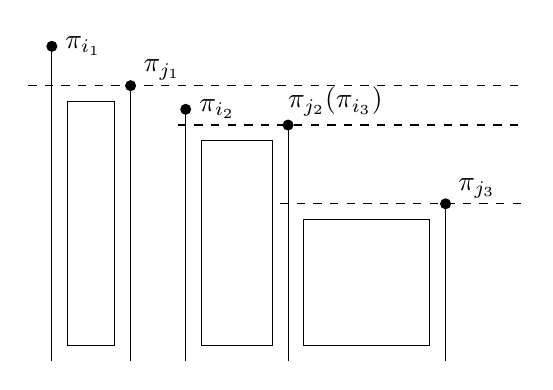
\begin{tikzpicture}
      \draw (0,0)--(0,4);
      \fill (0,4) circle[radius=2pt];
      \node at (0.4,4) {$\pi_{i_1}$};
      \draw (1,0)--(1,3.5);
      \fill (1,3.5) circle[radius=2pt];
      \node at (1.4,3.7) {$\pi_{j_1}$};
      \draw[dashed] (-0.3,3.5) -- (6,3.5);
      \draw (0.2,3.3) rectangle (0.8,0.2);

      \draw (1.7,0)--(1.7,3.2);
      \fill (1.7,3.2) circle[radius=2pt];
      \node at (2.1,3.2) {$\pi_{i_2}$};
      \draw (3,0)--(3,3);
      \fill (3,3) circle[radius=2pt];
      \node at (3.6,3.3) {$\pi_{j_2}(\pi_{i_3})$};
      \draw[dashed] (1.6,3) -- (6,3);
      \draw (1.9,2.8) rectangle (2.8,0.2);

      \draw (5,0)--(5,2);
      \fill (5,2) circle[radius=2pt];
      \node at (5.4,2.2) {$\pi_{j_3}$};
      \draw[dashed] (2.9,2) -- (6,2);
      \draw (3.2,1.8) rectangle (4.8,0.2);
    \end{tikzpicture}
    \caption{An illustration of choosing $\pi_{j_k}$ and $\pi_{i_k}$, $1\le k\le l$}
    \label{fig:312-4}
  \end{figure}

  The choices of $\pi_{i_k},\pi_{j_k}(1\le k \le l)$ imply that,  
  for all $1\le k \le l$, 
  \begin{enumerate}[label=(\roman*)]
      \item there is no $\underline{231}4$ pattern in $\pi_1\pi_2\cdots \pi_{n}$;
      \item $\pi_{i_k+1},\pi_{i_k+2},\cdots ,\pi_{j_k-1}<\pi_{j_k}<\pi_{i_k}$;
      \item there is no $\underline{312}4$ pattern in $\pi_{j_{k-1}+1}\pi_{j_{k-1}+2}\cdots \pi_{i_{k}}(j_{0}:=0)$;
      \item there must be a $\underline{312}4$ pattern in $\pi_{i_k+1} \pi_{i_k+2}\cdots \pi_{j_k}$;
      \item $j_k-i_k\ge 4$.
  \end{enumerate}
  Now we obtain the image permutation $f(\pi)$ from $\pi$ by keeping the positions and values of both $\pi_{i_k}$ and $\pi_{j_k}$, while transforming the subword $\pi_{i_k+1}\pi_{i_k+2}\cdots \pi_{j_{k}-1}$ to $\pi'_{i_k+1}\pi'_{i_k+2}\cdots \pi'_{j_k-1}$, for all $1\le k\le l$, where
  $\pi'_{i_k+1}\pi'_{i_k+2}\cdots \pi'_{j_k-1}$ is the permutation on
  $\{\pi_{i_k+1},\pi_{i_k+2},\cdots, \pi_{j_k-1}\}$ such that
  $$\std(\pi'_{i_k+1}\pi'_{i_k+2}\cdots \pi'_{j_k-1})=(\std (\pi_{i_k+1}\pi_{i_k+2}\cdots \pi_{j_k-1}))^{rc}.$$
  For instance, $f(867953124)=786952314$. Moreover, one should be able to verify the following facts for all $1\le k \le l$.
  \begin{enumerate}[label=(\roman*)]
      \item $\des(\pi)=\des(f(\pi))$ since $\pi_{i_k}$ and $\pi_{j_k}$ are greater than 
      the elements in \\ $\{\pi_{i_k+1},\pi_{i_k+2},\cdots, \pi_{j_k-1}\}$, and the composition $\phi_r\circ\phi_c$ preserves the descent number.
      \item all occurrences of $\underline{312}4$ in $\pi_{i_k+1} \pi_{i_k+2}\cdots \pi_{j_k}$ become occurrences of $\underline{231}4$ in $\pi_{i_k+1}' \pi_{i_k+2}'\cdots \pi_{j_k}'$.
      \item there is no $\underline{312}4$ pattern in $f(\pi)$.
      \item $\pi_{j_k}=f(\pi)_{j_k}$ is also the largest element of $B^{f(\pi)^{k-1}}$, where
      $B^{f(\pi)^{k-1}}$ is        
      the set of elements playing $``4"$ in each occurrence of $\underline{231}4$ in
      $$f(\pi)_{j_{k-1}+1}f(\pi)_{j_{k-1}+2}\cdots f(\pi)_{i_k} f(\pi)_{i_k+1}\cdots f(\pi)_{j_k-1} f(\pi)_{j_k}\cdots f(\pi)_n,\quad (f(\pi)^0:=f(\pi)).
      $$
      Moreover, $A^{\pi^k}=B^{f(\pi)^{k}}$ for all $0\le k \le l-1$ $(\pi^0=\pi,f(\pi)^{0}=f(\pi))$.
      \item there is no $\underline{231}4$ pattern in $\pi_{j_{k-1}+1}\pi_{j_{k-1}+2}\cdots \pi_{i_{k}}$.
  \end{enumerate}
  Therefore, $f(\pi)\in \S_n(\underline{312}4,\widecheck{\underline{231}4})$.

  To show that $f$ is invertible, the key thing to notice is that $f$ keeps the ``maximality" of $\pi_{j_k}(1\le k \le l)$. The inverse mapping $f^{-1}$ is constructed similarly as $f$, except now finding $\pi_{j_k}$ and $\pi_{i_k}$ is with respect to the pattern $\underline{231}4$,
  and we implement the same transformation on the subword $\pi_{i_k+1}\pi_{i_k+2}\cdots \pi_{j_{k}-1}$.
\end{proof}

\begin{remark}
  The bijection $f$ constructed in Theorem~\ref{312-4--231-4} also preserves the statistic $\inv $,
  i.e., $\inv (\pi)=\inv (f(\pi))$ for $\pi \in \S_n(\widecheck{\underline{312}4},\underline{231}4)$ since the composition $\phi_r\circ\phi_c$ preserves the number (and positions) of the inversion pairs, although their values are usually changed.
\end{remark}

We introduce two algorithms here to facilitate our proofs of the other equivalence classes.
Given a letter $a$ and a word $w$ so that $a$ is not contained in $w$.
The first algorithm \textit{REPLACEMENT-I} proceeds as follows.
\begin{enumerate}[label=(\arabic*)]
    \item Start with a pair $(a,w)$.
    \item \textbf{While} $a$ is larger than some element in $w$, \textbf{do} \label{Re2}
    \begin{enumerate}[label=(2.\arabic*)]
        \item Let $y$ be the largest element in $w$ smaller than $a$ and replace $y$ by $a$, get new $w$. \label{Re2.1}
        \item Set $a:=y$.
    \end{enumerate}
    \item Get new pair $(a,w)$ and \textbf{stop}.
\end{enumerate}
The \textit{REPLACEMENT-II} algorithm proceeds as follows.
\begin{enumerate}[label=(\arabic*)]
    \item Start with a pair $(a,w)$.
    \item \textbf{While} $a$ is smaller than some element in $w$, \textbf{do} \label{Re2-}
    \begin{enumerate}[label=(2.\arabic*)]
        \item Let $y$ be the smallest element in $w$ larger than $a$ and replace $y$ by $a$, get new $w$. \label{Re2.1-}
        \item Set $a:=y$.
    \end{enumerate}
    \item Get new pair $(a,w)$ and \textbf{stop}.
\end{enumerate}

\begin{proposition}
    When the pair $(a,w)$ is inputted, let $(a',w')$ and $(a'',w'')$ be the output pair after applying the \textit{REPLACEMENT-I} and \textit{REPLACEMENT-II} algorithms respectively, then 
    \begin{enumerate} %[label=\arabic*)]
        \item $a'$ is smaller than every element of $w'$, $a''$ is larger than every element of $w''$; 
        \item $\std(w')=\std(w)=\std(w'')$;
        \item $\des(w')=\des(w)=\des(w'')$.
    \end{enumerate}
\end{proposition}

\begin{proof}
  If $a'$ is larger than any element of $w'$, the step~\ref{Re2} of \textit{REPLACEMENT-I} needs to run for another round before the algorithm terminates, this proves the first property for $(a',w')$. The proofs of other properties should be straightforward and we omit them.
\end{proof}


\begin{theorem}
  We have the $\des$-Wilf equivalence $\underline{231}4 \overset{\des}{\sim }\underline{241}3$. \label{231-4--241-3}
\end{theorem}

\begin{proof}
  We construct a $\des$-preserving bijection
  $$g: \S_n(\underline{231}4,\widecheck{\underline{241}3}) \to \S_n(\widecheck{\underline{231}4},\underline{241}3).$$
  Suppose $\pi:=a_1a_2\cdots a_n\in \S_n(\underline{231}4,\widecheck{\underline{241}3})$. 
  Find all occurrences of $\underline{241}3$ in $\pi$, let $\{j_1,j_2,\ldots,j_l\}$
  be its indices for some $l$, i.e., $\std(a_{j_i}a_{j_i+1}a_{j_i+2})=231$ and there exists $p_i>j_i+2$
  such that $\std(a_{j_i}a_{j_i+1}a_{j_i+2}a_{p_i})=2413$ for all $1\le i \le l$.
  Without loss of generality, set $j_1<j_2<\cdots<j_l$, then $j_{i+1}-j_i\ge 2$ for all $1\le i < l$.
  We notice that since $\pi \in \mathfrak{S}_n(\underline{231}4)$, all of the elements after $a_{j_i+1}$ are smaller than $a_{j_i+1}$ for all $1\le i \le l$. In particular, $a_{j_1+1}>a_{j_2+1}>\cdots>a_{j_l+1}$.
    
  We execute the \textit{REPLACEMENT-I} algorithm on $(a_{j_1+1},a_{j_1+3}a_{j_1+4}\cdots a_n)$, but
  \begin{itemize}
      \item \textit{REPLACEMENT-I}~\ref{Re2} is modified to be ``$a$ is larger than some element which is larger than $a_{j_1}$ in $w$'';
      \item  and add the condition ``$y>a_{j_1}$'' to \textit{REPLACEMENT-I}~\ref{Re2.1}. 
  \end{itemize}
  Denote $\pi^1:=a_1^1\cdots a_{j_1}^1a_{j_1+1}^1a_{j_1+2}^1a_{j_1+3}^1 \cdots a_n^1$, where $(a_{j_1+1}^1,a_{j_1+3}^1a_{j_1+4}^1\cdots a_n^1)$ is the output from the above modified \textit{REPLACEMENT-I} algorithm while all remaining entries are the same as in $\pi$. One verifies that 
  \begin{enumerate}[label=(\roman*)]
      \item $\std(a_{j_1}^1a_{j_1+1}^1a_{j_1+2}^1a_{p_1}^1)=2314$ for some $p_1>j_1+2$;
      \item $\std(a_{j_1+3}^1 \cdots a_n^1)=\std(a_{j_1+3} \cdots a_n)$;
      \item $\des(\pi)=\des(\pi^1)$;
      \item there exists no $\underline{231}4$ pattern before $a_{j_1}^1$ of $\pi^1$;
      \item $a_{j_1+1}^1$ is the smallest element in $a_{j_1+3}a_{j_1+4}\cdots a_n$ such that $a_{j_1}<a_{j_1+1}^1<a_{j_1+1}$;
      \item there exists no $p_1>j_1+2$ such that $\std(a_{j_1}^1a_{j_1+1}^1a_{j_1+2}^1a_{p_1}^1)=2413$;
      \item $\std(a_{j_i}^1a_{j_i+1}^1a_{j_i+2}^1)=231$ and there exists $p_i>j_i+2$ such that $\std(a_{j_i}^1a_{j_i+1}^1a_{j_i+2}^1a_{p_i}^1)=2413$ for all $2\le i\le l$.
  \end{enumerate}
  Next, consider $a_{j_2}^1 a_{j_2+1}^1 a_{j_2+2}^1$, repeat the above operations by simply replacing the subscript $j_1$ with $j_2$ and the 
  superscript $1$ with $2$. Keep doing this for $a_{j_i}^{i-1} a_{j_i+1}^{i-1} a_{j_i+2}^{i-1}$ with $i=2,3,\ldots, l$ in that order. Set the image $g(\pi):=\pi^l$, the final output permutation after applying $l$ times of modified \textit{REPLACEMENT-I} algorithm. We see that there exists no $\underline{241}3$ patterns in $g(\pi)$. More precisely, all occurrences of $\underline{241}3$ in $\pi$ become occurrences of $\underline{231}4$ in $g(\pi)$.

  For example, $\underline{362}514 \mapsto 34\underline{261}5 \mapsto 342516$, and
  $\underline{462}513 \mapsto 45\underline{261}3 \mapsto 452316$. So $g(362514)=342516$, and $g(462513)=452316$.

  The construction of the inverse mapping $g^{-1}$ is straightforward. Observe that for all occurrences of $\underline{231}4$ in $g(\pi):=b_1b_2\cdots b_n$, its set of indices is still given by $\{j_1,j_2,\ldots,j_l\}$. That is to say, $\std(b_{j_i}b_{j_i+1}b_{j_i+2})=231$ and there exists $p_i>j_i+2$
  such that $\std(b_{j_i}b_{j_i+1}b_{j_i+2}b_{p_i})=2314$ for all $1\le i \le l$.
  We execute the suitably modified \textit{REPLACEMENT-II} algorithm on $(b_{j_l+1},b_{j_l+3}b_{j_l+4}\cdots b_n)$ to generate $(b_{j_l+1}^1,b_{j_l+3}^1b_{j_l+4}^1\cdots b_n^1)$, turning the $\underline{231}4$ occurrence beginning with $b_{j_l}b_{j_l+1}b_{j_l+2}$ into a $\underline{241}3$ occurrence beginning with $b_{j_l}b_{j_l+1}^1b_{j_l+2}$. Continue the process to replace the $\underline{231}4$ occurrences that begin with positions $j_{l-1},j_{l-2},\ldots,j_1$, in that order, until we finally arrive at a permutation that is in $\S_n(\underline{231}4,\widecheck{\underline{241}3})$, and it is taken to be the preimage $g^{-1}(b_1b_2\cdots b_n)$. For example, $34\underline{251}6\mapsto  \underline{342}615 \mapsto 362514 $, and $45\underline{231}6 \mapsto  \underline{452}613 \mapsto 462513$.
\end{proof}

Table~\ref{tab:231-4--241-3} lists the example of $\underline{231}4\overset{\des}{\sim} \underline{241}3$ for $n=5$.
The permutations in the same line are in correspondence with each other under our bijection $g$.

\begin{table}[h]
\setlength{\tabcolsep}{15pt}%调整列宽
  \renewcommand{\arraystretch}{1.2}
  \centering
  \begin{tabular}{ccc} 
      &  $\S_n(\underline{231}4,\widecheck{\underline{241}3})$ & $\S_n(\widecheck{\underline{231}4},\underline{241}3)$ \\ \hline
     %  & $\underline{241}35$ & $\underline{241}35$   \\
       & $\underline{251}34$ & $\underline{231}45$  \\
   $\mathrm{des}=1$    & $\underline{351}24$ & $\underline{341}25$  \\
       & $2\underline{351}4$ & $2\underline{341}5$  \\
       & $1\underline{352}4$ & $1\underline{342}5$  \\\hline
   %  & $\underline{241}53$ & $\underline{241}53$   \\
       & $5\underline{241}3$ & $5\underline{231}4$   \\
       & $\underline{251}43$ &  $\underline{231}54$ \\
       &  $3\underline{251}4$ &  $3\underline{241}5$ \\
        $\mathrm{des}=2$ & $4\underline{251}3$ &  $4\underline{231}5$ \\
       & $\underline{351}42$ & $\underline{341}52$  \\
       & $\underline{352}14$ & $\underline{342}15$  \\
       & $\underline{352}41$ & $\underline{342}51$  \\      
       \hline
  \end{tabular}
  \caption{$\underline{231}4\overset{\des}{\sim} \underline{241}3$ ($n=5$)}
  \label{tab:231-4--241-3}
\end{table}

\begin{theorem} \label{213-4--132-4}
  We have the $\des$-Wilf equivalence $\underline{213}4\overset{\des}{\sim }\underline{132}4$.
\end{theorem}

\begin{proof}
  We can prove $\underline{213}4\overset{\des}{\sim }\underline{132}4$ similarly using 
  the bijection $f$ from Theorem~\ref{312-4--231-4}, because ``4'' is the largest element in pattern
  $\underline{213}4$ and $(213)^{rc}=132$.
\end{proof}

\begin{theorem}
  We have the $\des$-Wilf equivalence $\underline{132}4\overset{\des}{\sim }\underline{142}3$. \label{132-4--142-3}
\end{theorem}

\begin{proof}
  The proof is analogous to that of Theorem~\ref{231-4--241-3}, we only need to transform all of the $\underline{132}4$ occurrences to $\underline{142}3$ occurrences. Note the following modifications to the \textit{REPLACEMENT-I} algorithm though:
  \begin{itemize}
      \item  the step~\ref{Re2} of \textit{REPLACEMENT-I} is modified to ``$a$ is larger than some element which is larger than $a_{j_1+2}$ in $w$'';
      \item  and add the condition ``$y>a_{j_1+2}$'' to \textit{REPLACEMENT-I}~\ref{Re2.1}. 
  \end{itemize}
  The inverse mapping and the \textit{REPLACEMENT-II} algorithm should be adjusted accordingly. We omit the details.
\end{proof}

\begin{theorem}
  We have the $\des$-Wilf equivalence $\underline{134}2 \overset{\des}{\sim } \underline{124}3$.  \label{134-2--124-3}   
\end{theorem}

\begin{proof}
  The same approach for proving Theorem~\ref{231-4--241-3} works for this pair as well. We want to transform all $\underline{134}2$ occurrences to $\underline{124}3$ occurrences, with the two algorithms modified as follows. For the forward mapping relying on \textit{REPLACEMENT-I},
  \begin{itemize}
      \item  \textit{REPLACEMENT-I}~\ref{Re2} is modified to ``$a$ is larger than some element which is larger than $a_{j_1}$ in $w$'';
      \item  and add the condition ``$y>a_{j_1}$'' to \textit{REPLACEMENT-I}~\ref{Re2.1}. 
  \end{itemize}
  For the backward mapping relying on \textit{REPLACEMENT-II}, 
  \begin{itemize}
      \item \textit{REPLACEMENT-II}~\ref{Re2-} is modified to ``$a$ is smaller than some element which is smaller than $a_{j_1+2}$ in $w$'';
      \item  and add the condition ``$y<a_{j_1+2}$'' to \textit{REPLACEMENT-II}~\ref{Re2.1-}. \qedhere
  \end{itemize}
\end{proof}

At this point, we have fully confirmed the fourteen $\des$-Wilf equivalence classes for quasi-consecutive patterns of length four; see Table~\ref{tab: descent vector of length 4}.


\section{Generating functions} \label{sec:g.f. of 4}

According to Theorem~\ref{structure thm}, we have the generating function for the quasi-consecutive pattern $\sigma k$, where $k$ is the largest element, provided the generating function for $\sigma$ is known. In this section, we derive an explicit generating function for one of the patterns, namely $\underline{123}$, and subsequently for $\underline{321}$ as well, thanks to Proposition~\ref{omega--omega^c}. The approach we use is the so-called generalized run theorem; see Theorem~\ref{thm:gen run thm}. For the remaining four patterns, $\underline{132}$, $\underline{213}$, $\underline{231}$, and $\underline{312}$, we demonstrate that their generating functions satisfy certain partial differential equations, as presented in Subsection~\ref{subsec:g.f.132}.

\subsection{The run theorem} \label{subsec:run theorem}


In this subsection we use Zhuang's generalized \emph{run theorem} \cite{zhu16} to get two generating functions. Here ``run'' refers to a maximal weakly increasing consecutive subsequence in a word, so naturally this theorem suits the increasing pattern $\underline{123}$ the best. But according to Proposition~\ref{omega--omega^c}, finding the Eulerian distribution over $\underline{123}$-avoiding permutations is equivalent to finding the Eulerian distribution over $\underline{321}$-avoiding permutations. And the bivariate generating function for $\underline{321}$-avoiding permutations is already known to be \cite{MR06}

\begin{align}\label{Sn321des}
	\sum_{n\geq 0}\dfrac{x^n}{n!}\sum_{\pi \in S_n(\underline{321})} t^{\mathrm{des}(\pi)}=\dfrac{\mathrm{e}^{x/2}\sqrt{1-4t}}{\sqrt{1-4t}\cosh {\left(\frac{x}{2}\sqrt{1-4t}\right)}-\sinh{\left(\frac{x}{2}\sqrt{1-4t}\right)}}.
\end{align}
See also \cite[Thm.~5.3.4]{kit11}. Our proof of the following result could thus be viewed as an alternative approach to deriving \eqref{Sn321des}. We only sketch a proof here using the run theorem and illustrate the associated ``run network'' in Fig.~\ref{sn123runnetwork}. To make the paper self-contained however, we provide some preliminary definitions and facts in the Appendix, and the reader is referred to Zhuang's original paper~\cite{zhu16} for further information.

Note that a permuation $\pi$ avoids the consecutive pattern $\underline{123}$ if and only if each run of $\pi$ has length 1 or 2. Therefore, the corresponding run network is given by Fig.~\ref{sn123runnetwork}.

% , and we assign the weights $w_1^{(1 , 1)}=w_2^{(1,1)}=t$.

\begin{figure}[htbp]	
	 \centering
		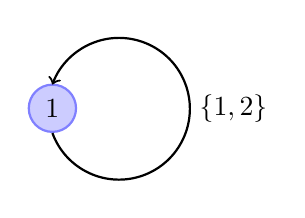
\begin{tikzpicture}
			[phase/.style ={circle,draw=blue!50,fill=blue!20,thick,inner sep=0pt, minimum size=6mm}]
			\node (A) at (0,-2) [phase] {1};
			\node (C) at (2.3,-2) {$\{1,2\}$};
			\draw[->,thick] (A.south) arc[start angle=-160, end angle=160, radius=9mm];
		\end{tikzpicture}
\caption{Run network for permutations avoiding consecutive pattern $\underline{123}$.}
\label{sn123runnetwork}
\end{figure}

\begin{theorem}
\begin{align}\label{Sn(123)des+1}
1+\sum_{n\geq 1}\dfrac{x^n}{n!}\sum_{\pi \in \S_n(\underline{123})} t^{\mathrm{des}(\pi)+1}=\dfrac{\mathrm{e}^{tx/2}\sqrt{t-4}}{\sqrt{t-4}\cosh {\left(\frac{x}{2}\sqrt{t^2-4t}\right)}-\sqrt{t}\sinh{\left(\frac{x}{2}\sqrt{t^2-4t}\right)}},
\end{align}
equivalently, we have
\begin{align}\label{Sn(123)des}
	\sum_{n\geq 0}\dfrac{x^n}{n!}\sum_{\pi \in \S_n(\underline{123})} t^{\mathrm{des}(\pi)}=\dfrac{t^{-1}\mathrm{e}^{tx/2}\sqrt{t-4}}{\sqrt{t-4}\cosh {\left(\frac{x}{2}\sqrt{t^2-4t}\right)}-\sqrt{t}\sinh{\left(\frac{x}{2}\sqrt{t^2-4t}\right)}}-\dfrac{1}{t}+1.
\end{align}
\end{theorem}

\begin{proof}
According to Fig.~\ref{sn123runnetwork} and applying Theorem~\ref{thm:gen run thm}, the inverse of $1+xt+x^2t$ is enumerator of those permutations whose increasing runs are no more than 2, and each increasing run is weighted by $t$. Next we proceed to seek the exponential generating function expression of $$\frac{1}{1+xt+x^2t}$$ with respect to the variable $x$. Since 
$$\dfrac{1}{1+xt+xt^2}=\dfrac{t-4+\sqrt{t^2-4t}}{2\left(t-4\right)}\dfrac{1}{1-\frac{2tx}{-t+\sqrt{t^2-4t}}}+\dfrac{t-4-\sqrt{t^2-4t}}{2(t-4)}\dfrac{1}{1-\frac{2tx}{-t-\sqrt{t^2-4t}}},$$ 
the exponential generating function turns out to be 
$$\frac{t-4+\sqrt{t^2-4t}}{2\left(t-4\right)} \mathrm{Exp}\left(\frac{-tx-x\sqrt{t^2-4t}}{2}\right)+\frac{t-4-\sqrt{t^2-4t}}{2\left(t-4\right)} \mathrm{Exp}\left(\frac{-tx+x\sqrt{t^2-4t}}{2}\right)$$
whose inverse simplifies to the desired expression \eqref{Sn(123)des+1}.
\end{proof}

% We note in passing that Eq.~\eqref{Sn(123)des} could be viewed as a bivariate extension of the expression of $P(0,z)$ in \cite[Thm.~4.1]{EN03}, which is the generating function of permutations avoiding $\underline{123}$.

%Note that $\pi^r \in \S_n(\underline{321})$ and $\mathrm{des}(\pi^r)=n-1-\mathrm{des}(\pi)$ if $\pi \in \S_n(123)$, consequently we have following result.
% By Proposition~\ref{omega--omega^c}, we immediately have the following result.
% \begin{corollary}	
% \begin{align}\label{Sn321des}
% 	\sum_{n\geq 0}\dfrac{x^n}{n!}\sum_{\pi \in S_n(\underline{321})} t^{\mathrm{des}(\pi)}=\dfrac{\mathrm{e}^{x/2}\sqrt{1-4t}}{\sqrt{1-4t}\cosh {\left(\frac{x}{2}\sqrt{1-4t}\right)}-\sinh{\left(\frac{x}{2}\sqrt{1-4t}\right)}}.
% \end{align}
% \end{corollary}


\subsection{The generating functions involving partial differential equations} \label{subsec:g.f.132}
Noting the equivalences implied by Proposition~\ref{omega--omega^rc}: $\underline{312} \overset{\des}{\sim }\underline{231} $, $\underline{213} \overset{\des}{\sim }\underline{132}$, and the relation $\underline{231}=(\underline{132})^r$, it suffices to compute the generating function for one of the patterns, say $\underline{132}$.

Let $U_n(t)$ (resp., $V_n(t)$) denote the generating function of the permutations $\pi$ of length $n$ that avoid the pattern $\underline{132}$ and start with an ascent $\pi_1 < \pi_2$ (resp., a descent $\pi_1 > \pi_2$), where $t$ tracks the descent number of $\pi$.
We define $U = U(x,t) := \sum_{n \geq 0} U_n(t) \frac{x^n}{n!}$ and $V = V(x,t) := \sum_{n \geq 0} V_n(t) \frac{x^n}{n!}$, with the initial terms given by $U_0(t) = U_1(t) = V_0(t) = V_1(t) = 0$.

\begin{proposition} \label{132}
The bivariate generating functions $U$ and $V$ satisfy the partial differential equations:
    \begin{align*}
    \dfrac{\partial U}{\partial x} &=(tU+1)(U+x+1)-1,\\
    \dfrac{\partial V}{\partial x} &=t(V+x)(U+x+1).
    \end{align*}
    Moreover,
    \begin{align*}
    A^{\underline{132}}(x,t)=A^{\underline{213}}(x,t)=1+x+U(x,t)+V(x,t).
    \end{align*}
\end{proposition}

\begin{proof}
    Let $\pi \in \S_{n+1}(\underline{132})$. Considering the position of $1$ as illustrated in Fig.~\ref{fig:position of 1}, we obtain
    \begin{equation}\label{eqn-prop-4-6}U_{n+1}(t)=tU_n(t)+tnU_{n-1}(t)+t\sum_{i=2}^{n-2}\binom{n}{i}U_i(t)U_{n-i}(t)+U_{n}(t),\quad n \ge 3.\end{equation}

    \begin{figure}[ht]
        \centering
        \begin{tikzpicture}
            \draw (0,0)--(5,0);
            \foreach \I in {0,0.5,...,5}
            {\draw (\I,0)--(\I,0.15);}
            \node at (4.75,0.3) {$1$};
        \end{tikzpicture}

        \begin{tikzpicture}
            \draw (0,0)--(5,0);
            \foreach \I in {0,0.5,...,5}
            {\draw (\I,0)--(\I,0.15);}
            \node at (4.25,0.3) {$1$};
        \end{tikzpicture}

        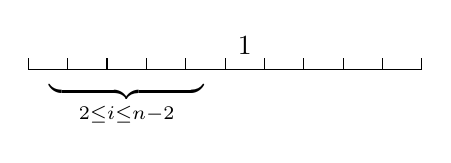
\begin{tikzpicture}
            \draw (0,0)--(5,0);
            \foreach \I in {0,0.5,...,5}
            {\draw (\I,0)--(\I,0.15);}
            \node at (2.75,0.3) {$1$};
            \node at (1.25,-0.3) {$\underbrace{\phantom{a+b+c+d}}_{2 \le i\le n-2}$ };
        \end{tikzpicture}

        \begin{tikzpicture}
            \draw (0,0)--(5,0);
            \foreach \I in {0,0.5,...,5}
            {\draw (\I,0)--(\I,0.15);}
            \node at (0.25,0.3) {$1$};
        \end{tikzpicture}
        \caption{Position of $1$ in $\pi \in \S_{n+1}(\underline{132})$}\label{fig:position of 1}
    \end{figure}
Multiplying by $\dfrac{x^n}{n!}$ both sides of (\ref{eqn-prop-4-6}) and summing over all $n\geq 3$, we have    

\begin{align*}
    \sum_{n\ge 3}U_{n+1}(t)\frac{x^n}{n!}={}&t\sum_{n\ge 3}U_n(t)\frac{x^n}{n!}+tx\sum_{n\ge 3}U_{n-1}(t)\frac{x^{n-1}}{(n-1)!} \\
    &+t\sum_{n\ge 3}\sum_{i=2}^{n-2}\binom{n}{i}U_i(t)U_{n-i}(t)\frac{x^n}{n!}+\sum_{n\ge 3}U_n(t)\frac{x^n}{n!} \\
    ={}& t\sum_{n\ge 3}U_n(t)\frac{x^n}{n!}+tx\sum_{n\ge 2}U_{n}(t)\frac{x^{n}}{n!} \\
    &+t\sum_{n\ge 3}\sum_{i=0}^{n}\binom{n}{i}U_i(t)U_{n-i}(t)\frac{x^n}{n!}+\sum_{n\ge 3}U_n(t)\frac{x^n}{n!} \\
    ={}& t\left(U-\frac{x^2}{2}\right)+txU+tU^2+\left(U-\frac{x^2}{2}\right).
\end{align*}

Note that $U_2(t)=1$ and $U_3(t)=1+t$. Hence,  
\begin{align*}
    \sum_{n\ge 3}U_{n+1}(t)\frac{x^n}{n!}&=\frac{\partial }{\partial x}\left(U-\frac{x^2}{2}-(1+t)\frac{x^3}{3!}\right) = \frac{\partial U}{\partial x}-x-(1+t)\frac{x^2}{2} \\
    &=t\left(U-\frac{x^2}{2}\right)+txU+tU^2+\left(U-\frac{x^2}{2}\right).
\end{align*}

Therefore, $\dfrac{\partial U}{\partial x}=x+tU+txU+tU^2+U=(tU+1)(U+x+1)-1$.
Using Mathematica, we obtain the expansion $U(x,t)=\dfrac{x^2}{2}+(1+t)\dfrac{x^3}{3!}+(1+5t+t^2)\dfrac{x^4}{4!}+(1+16t+10t^2+t^3)\dfrac{x^5}{5!}+(1+42t+71t^2+16t^3+t^4)\dfrac{x^6}{6!}+(1+99t+399t^2+197t^3+23t^4+t^5)\dfrac{x^7}{7!}+\cdots$.


Similarly, we have
$$V_{n+1}(t)=tV_n(t)+tnV_{n-1}(t)+t\sum_{i=2}^{n-2}\binom{n}{i}V_i(t)U_{n-i}(t)+tnU_{n-1}(t),\quad n\ge 3.$$
Note that $V_2(t)=t$ and $V_3(t)=2t+t^2$. Repeating the above computations for $V$, we have


\begin{align*}
    \sum_{n\ge 3}V_{n+1}(t)\frac{x^n}{n!}={}& t\sum_{n\ge 3}V_n(t)\frac{x^n}{n!}+tx\sum_{n\ge 3}V_{n-1}(t)\frac{x^{n-1}}{(n-1)!} \\
    &+t\sum_{n\ge 3}\sum_{i=2}^{n-2}\binom{n}{i}V_i(t)U_{n-i}(t)\frac{x^n}{n!}+tx\sum_{n\ge 3}U_{n-1}(t)\frac{x^{n-1}}{(n-1)!} \\
    ={}& t\sum_{n\ge 3}V_n(t)\frac{x^n}{n!}+tx\sum_{n\ge 2}V_{n}(t)\frac{x^{n}}{n!} \\
    &+t\sum_{n\ge 3}\sum_{i=0}^{n}\binom{n}{i}V_i(t)U_{n-i}(t)\frac{x^n}{n!}+tx\sum_{n\ge 2}U_{n}(t)\frac{x^{n}}{n!} \\
    ={} & t\left(V-\frac{tx^2}{2}\right)+txV+tUV+txU.
\end{align*}
Then,
\begin{align*}
    \sum_{n\ge 3}V_{n+1}(t)\frac{x^n}{n!} &= \frac{\partial }{\partial x}\left(V-t\frac{x^2}{2}-(2t+t^2)\frac{x^3}{3!}\right)=\frac{\partial V}{\partial x} -tx-tx^2\left(1+\frac{t}{2}\right) \\
    &=t\left(V-\frac{tx^2}{2}\right)+txV+tUV+txU.
\end{align*}

Therefore, $\dfrac{\partial V}{\partial x}=tx+tx^2+tV+txV+tVU+txU=t(V+x)(U+x+1)$.
Using Mathematica, $V(x,t)=t\dfrac{ x^2}{2}+(2t+t^2)\dfrac{x^3}{3!}+(3t+5t^2+t^3)\dfrac{x^4}{4!}+(4t+21t^2+9t^3+t^4)\dfrac{x^5}{5!}+\cdots$.
\end{proof}

\begin{corollary}\label{231}
We have
    \begin{align*}
    A^{\underline{231}}(x,t)=A^{\underline{312}}(x,t)=\dfrac{1}{t} \left(U(xt,\dfrac{1}{t})+V(xt,\dfrac{1}{t})\right)+x+1.
    \end{align*}
\end{corollary}

\begin{proof}
    Applying Proposition~\ref{omega--omega^c}, we obtain
    \begin{equation*}
    A^{\underline{231}}(x,t)=\dfrac{1}{t} \left(A^{\underline{132}}(xt,\dfrac{1}{t})-1\right)+1=\dfrac{1}{t} \left(xt+U(xt,\dfrac{1}{t})+V(xt,\dfrac{1}{t})\right)+1. \qedhere
    \end{equation*}
\end{proof}



\section{Conclusion}\label{conclusion}

This paper provides a complete $\des$-Wilf classification for quasi-consecutive patterns of length up to 4. Extending this classification to longer patterns would be interesting but may not be feasible with existing tools. Indeed, determining the descent distributions for consecutive patterns of length 4 or more is already a complex task, and even if successful, evaluating the integral in Theorem~\ref{id:struc} may not be possible. Nevertheless, descent distributions can still be studied over more restrictive sets of permutations, specifically when, in addition to avoiding a quasi-consecutive pattern, further constraints are imposed (e.g., avoidance of another pattern, a prescribed beginning or end of a permutation, etc.).

Finally, studying other permutation statistics, such as left-to-right and right-to-left minima and maxima  (see \cite{HK} for definitions), on permutations that avoid quasi-consecutive patterns would be an interesting direction for future research, extending our study of descents on such permutations.

\section{appendix}\label{sec:appendix}

To state the generalized run theorem, we start by introducing some definitions on words and compositions, then we review some basic facts about noncommutative symmetric functions. 

Given an alphabet $A$, the set of all words over $A$ is denoted by $A^*$, which is a free monoid under the operation of concatenation. If $A$ is a totally ordered set and $w \in A^*$, we call maximal weakly increasing consecutive subsequence in $w$ an \emph{increasing run} of $w$. It is clear that each word $w$ can be decomposed uniquely into a sequence of increasing runs. For example, let $\mathbf{P}$ denote the set of positve integers, then the word $w=73344256 \in \mathbf{P}^*$ is decomposed into three increasing runs, namely $7$, $3344$, and $256$.

Reall that for a permutation $\pi \in \S_n$, $\mathrm{Des}(\pi):=\{i \in [n-1]:\pi_i>\pi_{i+1}\}$ denotes the descent set of $\pi$. Clearly $\mathrm{Des}(\pi) \subseteq [n-1]$ and the lengths of increasing runs in $\pi$ from left to right constitute a composition of $n$. We call this composition the \emph{descent composition} of $\pi$, denoted as $\mathrm{Comp}(\pi)$. For example if $\pi=413782596$, then $\mathrm{Des}(\pi)=\{1,5,8\}$ and $\mathrm{Comp}(\pi)=\{1,4,3,1\}$. Obviously one can recover $\mathrm{Des(\pi)}$ from $\mathrm{Comp}(\pi)$ or the other way around. For $n\geq 1$ and $\pi \in \S_n$, we have $$|\mathrm{Comp}(\pi)|=\mathrm{des}(\pi)+1=|\mathrm{Des(\pi)}|+1.$$

Zhuang's generalized run theorem was developed to count words and permutations with restrictions on the lengths of their increasing runs.

Let $F$ be a field of characteristic zero. Denote by $F\left\langle\left\langle X_1, X_2, \ldots\right\rangle\right\rangle$ the $F$-algebra of formal power series in noncommuting variables $X_1, X_2, \ldots$. For $n \geq 1$, let

$$
\mathbf{h}_n:=\sum_{1 \leq i_1 \leq \cdots \leq i_n} X_{i_1} X_{i_2} \cdots X_{i_n}
$$and set $\mathbf{h}_0=1$. Then for any composition $L=\left(L_1, \ldots, L_l\right)$, let $\mathbf{h}_L:=\mathbf{h}_{L_1} \cdots \mathbf{h}_{L_l}$. The $F$-algebra $\mathbf{S y m}$ generated by the elements $\mathbf{h}_L$ is called the algebra of noncommutative symmetric functions with coefficients in $F$, which is a subalgebra of $F\left\langle\left\langle X_1, X_2, \ldots\right\rangle\right\rangle$. The vector space $\mathbf{S y m}_n$ of noncommutative symmetric functions homogeneous of degree $n$ is the span of the set $\left\{\mathbf{h}_L\right\}_{L \vdash n}$, where $L\vdash n$ means $L$ is a composition of $n$.

Next, we are going to introduce another base $\left\{\mathbf{r}_L\right\}_{L \vdash n}$ for the vector space of noncommutative symmetric functions homogeneous of degree $n$, see \cite{GKLLRT95} for more information about noncommutative symmetric functions. 

For any composition $L=\left(L_1, \ldots, L_l\right) \vdash n$, let

$$
\mathbf{r}_L:=\sum_{\left(i_1, \ldots, i_n\right)} X_{i_1} X_{i_2} \cdots X_{i_n}
$$where the sum is over all $\left(i_1, \ldots, i_n\right)$ satisfying

$$
\underbrace{i_1 \leq \cdots \leq i_{L_1}}_{L_1}>\underbrace{i_{L_1+1} \leq \cdots \leq i_{L_1+L_2}}_{L_2}>\cdots>\underbrace{i_{L_1+\cdots+L_{l-1}+1} \leq \cdots \leq i_n}_{L_l} .
$$

Define a partial order ``$\leq$'' on the set of compositions of $n$ by reverse refinement, that is, $K=\left(K_1, \ldots, K_k\right) \vdash n$ covers $L$ if and only if $L$ can be obtained from $K$ by replacing two consecutive parts $K_i$ and $K_{i+1}$ with $K_i+K_{i+1}$. It is easy to see that 


$$
\mathbf{h}_L=\sum_{K \leq L} \mathbf{r}_K.
$$Thus, by inclusion-exclusion we have

$$
\mathbf{r}_L=\sum_{K \leq L}(-1)^{\#L-\#K} \mathbf{h}_K,
$$where $\#L$ denotes the number of parts in $L$. Note that the functions $\mathbf{h}_L$ and $\mathbf{r}_L$ are noncommutative versions of the \emph{complete symmetric functions} and the \emph{ribbon Schur functions} (see \cite[Chap.~7]{sta11}), respectively.

Define the homomorphism $\Phi: \mathbf{S y m} \rightarrow F[[x]]$ by $\Phi\left(\mathbf{h}_n\right)=\dfrac{x^n}{n!}$. Then, $$\Phi(\mathbf{h}_{L})=\frac{x^{L_1}}{L_1 !}\cdots \frac{x^{L_l}}{L_l !}=\binom{n}{L}\frac{x^n}{n!},$$
where we use the abbreviation for multinomial coefficient $\binom{n}{L}:=\binom{n}{L_1,\ldots,L_l}$. Although noncommutative symmetric functions are generating functions for words, the following lemma allows us to move from the realm of word enumeration to that of permutation enumeration.

\begin{lemma}{\cite{zhu17}}
For a given composition $L\vdash n$, we have  
\begin{equation}\label{homomorphsim}
\Phi (\mathbf{r}_L)=\sum_{\substack{\pi \in \S_n\\ \mathrm{Comp}(\pi)=L}} \frac{x^n}{n!}
\end{equation}
\end{lemma}

\begin{Def}{(\emph{run network})} A digraph $G$ on vertex set $[m]$ where each arc $(i, j)$ is assigned a nonempty subset $P_{i, j} \subseteq \mathbf{P}$ is called a network of order $m$. Given such a network, let $P$ be the set of all pairs $(a, e)$ such that $a \in P_{i, j}$ and $e=(i, j)$ is an arc of $G$. Furthermore, let $\overrightarrow{P^*} \subseteq P^*$ be the subset of all sequences $\alpha=\left(a_1, e_1\right)\left(a_2, e_2\right) \cdots\left(a_n, e_n\right)$ such that $e_1 e_2 \cdots e_n$ is a walk in $G$.

Let $(G, P)$ be a network of order $m$ with $\overrightarrow{P^*}$ as constructed above. For $\alpha=\left(a_1, e_1\right) \cdots\left(a_n, e_n\right) \in \overrightarrow{P^*}$ with $i$ and $j$ respectively the initial and terminal vertices of the walk $e_1 \cdots e_n$, let $\rho(\alpha)=\left(a_1, a_2, \ldots, a_n\right)$ and $E(\alpha)=(i, j)$. Then $(G, P)$ is a run network of order $m$ if for any $\alpha, \beta \in \overrightarrow{P^*}$, whenever $\rho(\alpha)=\rho(\beta)$ and $E(\alpha)=E(\beta)$, there is $\alpha=\beta$. In other words, the same tuple $\left(a_1, a_2, \ldots, a_n\right)$ cannot be obtained by traversing two different walks in $G$ with the same initial and terminal vertices.
\end{Def}


\begin{theorem}{(Generalized Run Theorem~\cite{zhu17})}\label{thm:gen run thm}
  Suppose that $(G, P)$ is a run network of order $m$ and $A$ is a unital $F$-algebra of characteristic zero. Let $\left\{w_a^{(i , j)}:(a,(i, j)) \in P\right\}$ be a set of weights from $A$, with $w_a^{(i, j)}=0$ if $(a,(i, j)) \notin P$. For a composition $L=\left(L_1, \ldots, L_l\right)$ and $i, j \in[m]$, let $w^{(i, j)}(L)=w_{L_1}^{e_1} \cdots w_{L_l}^{e_l}$ if there exists $\alpha=\left(L_1, e_1\right) \cdots\left(L_l, e_l\right) \in \overrightarrow{P^*}$ such that $E(\alpha)=(i, j)$ and $L=\rho(\alpha)$, and let $w^{(i, j)}(L)=0$ otherwise. Let $v_n^{(i, j)}$ be defined by
    
\begin{align*}
      \left[\begin{array}{ccc}
      \sum\limits_{n \geq 0} v_n^{(1,1)} x^n & \cdots & \sum\limits_{n \geq 0} v_n^{(1, m)} x^n \\
      \vdots & \ddots & \vdots \\
      \sum\limits_{n \geq 0} v_n^{(m, 1)} x^n & \cdots & \sum\limits_{n \geq 0} v_n^{(m, m)} x^n
  \end{array}\right]=\left(I_m+\left[\begin{array}{ccc}
      \sum\limits_{k \geq 1} w_k^{(1,1)} x^k & \cdots & \sum\limits_{k \geq 1} w_k^{(1, m)} x^k \\
      \vdots & \ddots & \vdots \\
      \sum\limits_{k \geq 1} w_k^{(m, 1)} x^k & \cdots & \sum\limits_{k \geq 1} w_k^{(m, m)} x^k
  \end{array}\right]\right)^{-1},
\end{align*}

  where $I_m$ denotes the $m \times m$ identity matrix. Then
    
  \begin{align}
      \left[\begin{array}{ccc}\label{nonComGen}
      \sum\limits_L w^{(1,1)}(L) \mathbf{r}_L & \cdots & \sum\limits_L w^{(1, m)}(L) \mathbf{r}_L \\
      \vdots & \ddots & \vdots \\
      \sum\limits_L w^{(m, 1)}(L) \mathbf{r}_L & \cdots & \sum\limits_L w^{(m, m)}(L) \mathbf{r}_L
  \end{array}\right]=\left[\begin{array}{ccc}
      \sum\limits_{n \geq 0} v_n^{(1,1)} \mathbf{h}_n & \cdots & \sum\limits_{n \geq 0} v_n^{(1, m)} \mathbf{h}_n \\
      \vdots & \ddots & \vdots \\
      \sum\limits_{n \geq 0} v_n^{(m, 1)} \mathbf{h}_n & \cdots & \sum\limits_{n \geq 0} v_n^{(m, m)} \mathbf{h}_n
  \end{array}\right]^{-1},
  \end{align}

    
  where each sum in the matrix on the left-hand side is over all compositions $L$.
\end{theorem}

\section*{acknowledgement}
We are grateful to Quan Yuan for her help in finding the $\des$-Wilf-equivalence classifications
for quasi-consecutive patterns of length $4$. 


\begin{thebibliography}{99}
%    \bibitem{bax14} A.~M.~Baxter, Refining enumeration schemes to count according to permutation statistics, {\em Electron. J. Combin.} {\bf21} (2014), \#P2.50.

    \bibitem{BP12} A.~M.~Baxter and L.~K.~Pudwell, Enumeration schemes for vincular patterns, {\em Discrete Math.} {\bf312} (2012), 1699--1712.

    \bibitem{BS15} A.~M.~Baxter and M.~Shattuck, Some Wilf-equivalences for vincular patterns, {\em J. Comb.} {\bf6} (2015), 19--45.

    \bibitem{BDGZ19}C. Bielawa, R. Davis, D. Greeson and Q. Zhou, Descents and des-Wilf equivalence of permutations avoiding certain nonclassical patterns, {\em Involve} \textbf{12} (2019), 549--563. 

    \bibitem{Bukata2019}
    M. Bukata, R. Kulwicki, N. Lewandowski, L. Pudwell, J. Roth, T.	Wheeland. Distributions of statistics over pattern-avoiding permutations. {\em J. Integer Sequences} {\bf 22} (2019) Article 19.2.6.

    \bibitem{CN18} E.~Chen and S.~Narayanan, The 26 Wilf-equivalence classes of length five quasi-consecutive patterns, {\em Discrete Math. Theor. Comput. Sci.} {\bf20} (2018), \#12.
    
    \bibitem{cla01}A. Claesson, Generalized pattern avoidance, {\em European J. Combin.} \textbf{22} (2001), 961--971.

    \bibitem{eli06} S.~Elizalde, Asymptotic enumeration of permutations avoiding generalized patterns, {\em Adv. Appl. Math.} {\bf36} (2006), 138--155.
    
    \bibitem{eliz16} S.~Elizalde, A survey of consecutive patterns in permutations, {\em IMA Vol. Math. Appl.} {\bf 159}, Springer, [Cham], 2016. 

%    \bibitem{EN03} S. Elizalde and M. Noy, Consecutive patterns in permutations, {\em Adv. Appl. Math.} \textbf{30} (2003), 110--125.
    \bibitem{FS70} D.~Foata and M.-P.~Sch\"utzenberger, {\it Th\'eorie g\'eom\'etrique des polyn\^omes eul\'eriens}, Lecture Notes in Mathematics, {\bf138}, Berlin, Springer (1970).

    \bibitem{FTHZ19} S. Fu, D. Tang, B. Han and J. Zeng, $(q,t)$-Catalan numbers: gamma expansions, pattern avoidances, and the $(-1)$-phenomenon, {\em Adv. Appl. Math.} \textbf{106} (2019), 57--95.

   \bibitem{GKLLRT95}I.M. Gelfand, D. Krob, A. Lascoux, B. Leclerc, V.S. Retakh, and J.Y. Thibon, Noncommutative symmetrical functions, {\em Adv. Math.} \textbf{112} (1995), 218--348.

\bibitem{HK} T. Han and S. Kitaev, Joint distributions of statistics over permutations avoiding two patterns of length 3, {\em Discr. Math. and Theor. Comput. Sci.} {\bf 26:1}, Permutation Patterns 2023, (2024),  \#4 .

    \bibitem{kit05} S.~Kitaev, Partially ordered generalized patterns, {\em Discr. Math.} {\bf298} (2005), 212--229.
    
    \bibitem{kit11} S. Kitaev, {\it Patterns in Permutations and Words}, Springer Berlin, Heidelberg (2011).
    
    \bibitem{knu75} D. E. Knuth, {\it The art of computer programming, vol. 1, Fundamental Algorithms, 2nd edition}, Addison-Wesley Series in Computer Science and Information Processing, Addison-Wesley (1975).  
    
    \bibitem{mac60} P. A. MacMahon, {\it Combinatory analysis}, Chelsea, New York (1960).

    \bibitem{MR06} A. Mendes and J. Remmel, Permutations and words counted by consecutive patterns, {\em Adv. Appl. Mathem.} {\bf37} (2006), 443--480.
    
    \bibitem{pet15}T. K. Petersen, {\it Eulerian Numbers}, Birkh\"auser, New York (2015).

    \bibitem{rei95} V.~Reiner, The distribution of descents and length in a Coxeter group, {\em Electron. J. Combin.} {\bf2} (1995), R25.

    \bibitem{rio58} J.~Riordan, {\it An introduction to combinatorial analysis}, New York, Wiley (1958).

    \bibitem{sag91} B. E.~Sagan, {\it The symmetric group: representations, combinatorial algorithms, and symmetric functions}, Wadsworth (1991).

    \bibitem{SS85} R. Simion and F. W. Schmidt, Restricted permutations, {\em European J. Combin.} \textbf{6} (1985), 383--406.
    
    \bibitem{sta11}R. Stanley, { \it Enumerative Combinatorics}, Vol. 1, 2nd edition, Cambridge Studies in Advanced Mathematics, Cambridge University Press (2011). 
    
    \bibitem{zhu16}Y. Zhuang, Counting permutations by runs, {\em J. Combin. Theory Ser. A} \textbf{142} (2016), 147--176.
    
   \bibitem{zhu17}Y. Zhuang, Eulerian polynomials and descent statistics, {\em Adv. Appl. Math.} \textbf{90} (2017), 86--144.
    
\end{thebibliography}









\end{document}

